\documentclass[10pt,usenames,dvipsnames]{article}

\usepackage{amsmath}
\usepackage{amssymb}
\usepackage{amsthm}
\usepackage{bm}
\usepackage{bbm}
\usepackage{mathtools}
\usepackage{enumitem}
\usepackage[margin=1.25in]{geometry}
\usepackage[T1]{fontenc}
\usepackage{kpfonts}
\usepackage{mathpartir}
\usepackage{subfigure}
\usepackage{listings}
\usepackage{xcolor}
\usepackage{xspace}
\usepackage{tikz}
\usepackage{tkz-euclide}

\usepackage[
backend=biber,
style=numeric,
sorting=nty]{biblatex}

\addbibresource{biblio.bib}

\usepackage{hyperref}
\hypersetup{
    colorlinks=true,
    linkcolor=blue,
    filecolor=magenta,      
    urlcolor=blue,
}

\author{Reed Oei, Eric Ma, Tatum Schmidt, Abdullah Dean, \\Christian Schulz, Philipp Hieronymi}

\usepackage{graphicx}
\graphicspath{ {./images/} }

\input{Pecan/pecan-lang.tex}
%\newcommand{\reed}[1]{\relax}
%\newcommand{\eric}[1]{\relax}
%\newcommand{\christian}[1]{\relax}
%\newcommand{\philipp}[1]{\relax}
%\newcommand{\Fix}[1]{\relax}
\newcommand{\reed}[1]{{\color{magenta}\bfseries [#1]}}
\newcommand{\eric}[1]{{\color{green}\bfseries [#1]}}
\newcommand{\christian}[1]{{\color{orange}\bfseries [#1]}}
\newcommand{\philipp}[1]{{\color{blue}\bfseries [#1]}}
\newcommand{\Fix}[1]{{\color{red}\bfseries [#1]}}
\newcommand{\Comment}[1]{}
\newcommand{\Space}[1]{}
\newcommand{\Num}[1]{#1}

\newcommand{\term}[1]{\emph{#1}}

\newcommand{\Free}{\textbf{Free}}

\newcommand{\evaluates}{\Downarrow}

\newcommand{\R}{\mathbb{R}}
\newcommand{\Q}{\mathbb{Q}}
\newcommand{\Z}{\mathbb{Z}}
\newcommand{\N}{\mathbb{N}}

\newcommand{\join}{\wedge}
\newcommand{\meet}{\vee}
\newcommand{\proves}{\vdash}

\newcommand{\dom}{\text{dom}~}

\newcommand{\proj}{\text{proj}}

\newcommand{\implicits}{\texttt{implicit}}
\newcommand{\params}{\texttt{params}}
\newcommand{\nonvar}{\texttt{nonvar}}

\newcommand{\tand}{\ensuremath{~\text{and}~}}
\newcommand{\tor}{\ensuremath{~\text{or}~}}
\newcommand{\twhere}{\ensuremath{~\text{where}~}}
\newcommand{\tif}{\ensuremath{~\text{if}~}}
\newcommand{\tsuchthat}{\ensuremath{~\text{s.t.}~}}
\newcommand{\owise}{\ensuremath{~\text{otherwise}~}}

\newcommand{\brackets}[3]{\ensuremath{{\left#1 {#3} \right#2}}}
\newcommand{\parens}[1]{\brackets{(}{)}{#1}}
\newcommand{\angles}[1]{\brackets{<}{>}{#1}}
\newcommand{\curlys}[1]{\brackets{\{}{\}}{#1}}
\newcommand{\squares}[1]{\brackets{[}{]}{#1}}

\newcommand{\bnfdef}{\ensuremath{\Coloneqq}}
\newcommand{\bnfalt}{\ensuremath{\mid}\xspace}

\newcommand{\inferred}{\texttt{Inferred}}
\newcommand{\prop}[1]{#1 ~ \text{prop}}
\newcommand{\typ}[1]{\text{typ}\parens{#1}}


\title{Pecan \\
    \large An Automated Theorem Prover}
\begin{document}

\maketitle

\section{Introduction}

\textbf{Pecan} is a system for \emph{automated theorem proving} originally designed to decide mathematical statements about families of infinite words, in particular about Sturmian words, and based on well-known decision procedures for B\"uchi automata due to B\"uchi \cite{Buechi}. Pecan is inspired by Walnut~\cite{walnut} by Mousavi, another automated theorem prover for deciding combinatorical properties of automatic words. \textbf{Automatic words} are sequences of terms characterized by finite automata. The main motivation to create this new tool is to decide whether a statement is true for every element of an infinite family of words rather than just determining the truth of the statement for a single given words. In such a situation not every word in this family of words is automatic, but the whole family can be recognized by an automaton.
Since the infinite families of words we want to consider are often indexed by real numbers, it is convenient to work with B\"uchi automata instead of finite automata. The canonical example of such a automatic family of words are the \textbf{Sturmian words}, that is the family $(\mathbf{w}_{\alpha,\rho})$ of all words $w=(w_n)$ over the alphabet $\{0,1\}$ such that there is $\rho \in [ 0,1 )$, called the \emph{intercept}, and an irrational $\alpha \in (0,1)$, called the \emph{slope}, with
\[
w_{n}=\lfloor n\alpha +\rho\rfloor -\lfloor (n-1)\alpha +\rho\rfloor
\]
for all $n\in \N$. Using Pecan, we can automatically reprove classical and recent theorems about Sturmian words, like the fact that they are not periodic, within minutes, and even have been able to prove completely new mathematical theorems using this software. 

The idea of using automata-based decision procedures to prove theorems in combinatorics on words has been championed by Jeffrey Shallit and successfully implemented in several papers of Shallit and his many co-authors (see Shallit \cite{Shallit-survey} for a survey and Baranwal, Schaeffer, Shallit \cite{BARANWAL2021} for implementations of decision procedure for individual Sturmian words). The development of Pecan is our contribution to this exciting research program. We leave the detailed discussion of the mathematical background such as why Sturmian words can represented using automata and which statements about Sturmian words can be proved using Pecan, to the upcoming paper \cite{DecStuWor}. Here we describe the implementation of Pecan and discuss its performance.

% Pecan comes with \textbf{Praline}\footnote{Because it is syntactic \textbf{sugar} for Pecan.}, a scripting language designed to make working with Pecan more pleasant.
% It provides the primary interface to the counterexample generation capabilities of Pecan, and also allows some degree of metaprogramming: for example, programmatically generating predicate definitions.

\begin{subsection}{Related work} 
Pecan improves on Walnut~\cite{walnut}, a similar automata-based theorem prover for automatic sequences, by using B\"uchi automata instead of finite automata.
This difference enables Pecan to handle uncountable families of sequences, allowing us quantify over all Sturmian words. Additionally, the Pecan language is able to use multiple numeration systems at a time, has a concept of types outside of numeration systems, and has meta-programming language, Praline.

Many other theorem provers exist, such as SMT solvers and proof assistants, like Coq~\cite{the_coq_development_team_2020_3744225} or Isabelle~\cite{nipkow2002isabelle}.
To our knowledge, no SMT solver supports reasoning about Sturmian words.
Systems like Coq or Isabelle have projects attempting to formalize some aspects of combinatorics on words and automatic sequences~\cite{hivert2018littlewoodrichardson,holub2020binary}.
However, proofs in these systems are mostly human written, with some help from heuristics or specialized solvers, rather than being fully automatic, as in Pecan.

B\"uchi automata have also been used extensively in program verification in systems such as SPIN~\cite{gerard2003spin}.
However, we are interested in proving mathematical results, rather than proofs about properties of programs.
For this reason, we must allow unrestricted use of logical operations, such as negation, rather than restricting to more limited forms of expressing properties, such as linear temporal logic, which such systems tend to use for performance reasons.

\end{subsection}

\begin{subsection}{Acknowledgements}
Support for this project was provided by the Illinois Geometry Lab. This project was partially supported by NSF grant DMS-1654725. \end{subsection}
\section{Background}\label{sec:background}

This section contains an informal introduction to words, automata, and the notation that we use.
For precise statements and proof, we refer the reader to Allouche and Shallit \cite{MR1997038} or Khoussainov and Nerode ~\cite{aut_theory}.

Let $\Sigma^*$ denote the set of finite words on the alphabet $\Sigma$, let $\Sigma^+$ denote the set of nonempty finite words on the alphabet $\Sigma$, and let $\Sigma^\omega$ denote the set of $\omega$-words on the alphabet $\Sigma$.

For a word $w$, let $w[i]$ denote the $i$-letter of $w$.
Let $w(i,n)$ denote the length-$n$ factor of $w$ starting at $i$ and ending at $i + n - 1$, that is, $w[i \ldots i + n - 1] = w[i] w[i + 1] \cdots w[i + n - 1]$.
Let $|w|$ denote the \term{length} of $w$.
%Let $w^R$ denote the \term{reverse} of $w$, so if $w = w[1] w[2] \cdots w[n]$, then $w^R = w[n] w[n-1] \cdots w[1]$.
%In a binary alphabet, $\Sigma = \{0,1\}$, for a symbol $x \in \Sigma$, let $\overline{x}$ denote the \term{complement} of $x$, so $\overline{0} = 1$ and $\overline{1} = 0$.
%For a word $w$ over a binary alphabet, let $\overline{w}$ denote the \term{complement} of $w$, that is $\overline{w} = \overline{w[1]} \, \overline{w[2]} \cdots \overline{w[n]}$.
%Let $w^n$ denote concatenating $w$ with itself $n$ times, i.e., $w^n = \overbrace{w \cdots w}^{n\text{ times}}$.

\term{B\"uchi automata} are an extension of the standard finite automata to infinite inputs.
A B\"uchi automata $\mathcal{A} = (Q, \Sigma, \delta, q_0, F)$ accepts an infinite word $w \in \Sigma^\omega$ if the run of the automaton on the word $w$ visits an accepting state (i.e., a state in $F$) infinitely many times.
The set of words accepted by $\mathcal{A}$ is its \term{language}, $L(\mathcal{A})$.
Notably, nondeterministic B\"uchi automata and \textbf{not} equivalent to deterministic B\"uchi automata, and many interesting properties are only expressible via nondeterministic B\"uchi automata.
For that reason, we simply refer to nondeterministic B\"uchi automata as B\"uchi automata, without qualification.
Additionally, when we say ``automata'' without qualification, we refer to B\"uchi automata.
Importantly, the languages that B\"uchi automata define are closed under intersection, union, projection, and complementation, and emptiness checking is decidable.

%\cite{BARANWAL2021}
%Informally, a binary sequence $(a_n)_{n \in \N}$ is \term{automatic} if there is some automaton $\mathfrak{A}$ such that $a_n = 1$ if and only if $\rho(n) \in L(\mathfrak{A})$, where $\rho : \N \to \Sigma^*$ is a function mapping natural numbers to their representations in some numeration system. For example, $\rho$ might map natural numbers into their $k$-ary representations. In this case, we call the sequence $(a_n)_{n\in \N}$ $k$-automatic. 




% Using B\"uchi automata has a number of advantages over finite automata:
% \begin{itemize}
%         \item Some problems are more naturally expressed with B\"uchi automata.
%             For example, we think of numbers as having infinitely many leading/leading zeros; using B\"uchi automata, we can encode number so that they actually start with infinitely many zeros.
%             While existential quantification for Pecan works the same regardless of input type, Walnut needs a special algorithm to handle these leading/tailing zeroes because it uses finite automata.
            
%         \item Some problems can \emph{only} be expressed with B\"uchi automata.
%             For example, it is clearly impossible to encode real numbers as finite strings because there are uncountably many real numbers but only countably many finite strings (on a finite alphabet).
%             However, using B\"uchi automata, we are able to automatically prove properties about real numbers.
        
%         \item We can still express properties about finite strings (e.g., by using some symbol as an ``end of input'').
% \end{itemize}

% There are also disadvantages to using B\"uchi automata: in particular, many of the algorithms implementing the various logical operations on B\"uchi automata are much slower than their finite automata counterparts.
% For example, while complementing finite automata is simple, complementing B\"uchi automata requires exponential time.
% In practice, however, we can often calculate complements, even of large automata, in reasonable amounts of time.


\section{Usage}\label{sec:usage}

To install Pecan see the instructions at \url{https://github.com/ReedOei/Pecan}.

\subsection{Running Pecan}

The standard method of using Pecan is to create a new file (with a \texttt{.pn} extension) which will hold all definitions and theorems.
Then the file can be run using the following command on most operating systems (whether you use \texttt{python3} or \texttt{python} depends on how Python is installed):

\begin{lstlisting}[language=bash, basicstyle=\normalsize\ttfamily]
$ python3 pecan.py FILENAME
\end{lstlisting}

You can also run the file in \textbf{interactive mode}, which will run the file and then allow you to directly type new definitions and directives with the definitions from the file loaded:

\begin{lstlisting}[language=bash, basicstyle=\normalsize\ttfamily]
$ python3 pecan.py -i [FILENAME]
\end{lstlisting}

\subsection{A First Theorem}

For a taste of Pecan's syntax and the sort of theorems we can prove using Pecan, we'll prove a simple theorem about natural numbers:

\begin{theorem}
Every natural number is either even or odd.
\end{theorem}

Pecan has a built-in definition of natural numbers, which we will use to write a definition of ``even'' for natural numbers \footnote{Pecan also has an \texttt{even} predicate in its standard library, called \texttt{even}, however, we will write our own for instruction purposes.}.
The primary method of defining predicates in Pecan is the following:

\begin{pecan}
PREDICATE_NAME(ARGUMENTS) := BODY
\end{pecan}

In our particular case, we can define a number to be even if there is another number that is half of it.
We write this definition in Pecan as:

\begin{pecan}
is_even(x is nat) := existsy is nat. x = 2*y
\end{pecan}

Let's unpack this definition a little.
First, we say that \pecaninline{x is nat} in the arguments of \pecaninline{is_even} so that Pecan knows the \textbf{type} of the arguments, and we do the same on the existential quantifier for \pecaninline{y}.
Specifying the type allows Pecan to lookup the appropriate arithmetic operator definitions (e.g., for addition).
You can think of \pecaninline{x is nat} as being equivalent to $x \in \N$.
The body of the predicate, \pecaninline{existsy is nat. x = 2*y} works almost exactly like in a standard mathematical definition; \pecaninline{is_even(x)} is true if and only if \pecaninline{existsy is nat. x = 2*y}.

Note that instead of writing \pecaninline{x is nat} all the time, we can \textbf{restrict} certain variables to only be a specific type using the \pecaninline{Restrict} directive.
Let's do that for a few variables:

\begin{pecan}
Restrict x,y,z are nat.
\end{pecan}

Note that above \pecaninline{are} is just another way to write \pecaninline{is}.
We can get an example of a number that this predicate accepts with the following line.

\begin{pecan}
Example using natFormat of { is_even(x) }.
\end{pecan}

\begin{pecan_output}
[(x,0)]
\end{pecan_output}

That is, one input that \pecaninline{is_even} accepts is $0$, which makes sense, because $0$ is a natural number and $0$ is even.
Natural numbers in Pecan are, by default, in LSD (least-significant digit first) format, which is the reverse of the standard order; this order makes the underlying implementation significantly easier.
We can ask Pecan for more interesting examples as well.
For example, we can ask for an odd number greater than 33 by writing the following:

\begin{pecan}
is_odd(x) := existsy. x = 2*y+1
Example using natFormat of { x > 33 & is_odd(x) }.
\end{pecan}

We omitted the \pecaninline{x is nat} and \pecaninline{y is nat}; this omission is allowed because of the restriction we placed on \pecaninline{x} and \pecaninline{y}.
When we run the file, Pecan responds with:

\begin{pecan_output}
[(x,49)]
\end{pecan_output}

Again, this answer makes sense: it is an odd number, and it is greater than 33.
This particular feature is non-deterministic---you may not get the same examples inputs that we show here.
Also note that this output has been pretty-printed---if you want the raw input string, which will be an infinite binary string, you can instead use:

\begin{pecan}
Example using stdFormat of { x > 33 & is_odd(x) }.
\end{pecan}

This command gives me \pecaninline{[(x,100011(0)^w)]}, meaning that the input string starts with \pecaninline{100011} and then is \pecaninline{0} repeated infinitely many times.

Now that we've explored Pecan a little bit, let's write the actual theorem, and ask Pecan to check it.

\begin{pecan}
Theorem ("All natural numbers are even or odd", {
    forallx. is_even(x) | is_odd(x)
}).
\end{pecan}

Pecan proves the theorem is true, which the following output indicates.

\begin{pecan_output}
[INFO] Checking if All natural numbers are even or odd is true.
$\text{\color{ForestGreen}All natural numbers are even or odd is true.}$
\end{pecan_output}

We can see this theorem is true in another way, by confirming that a natural number is odd if and only if it is not even.

\begin{pecan}
Theorem ("x is odd if and only if it is not even", {
    forallx. is_odd(x) <=> !is_even(x)
}).
\end{pecan}

Again, Pecan confirms this theorem:

\begin{pecan_output}
[INFO] Checking if x is odd if and only if it is not even is true.
$\text{\color{ForestGreen}x is odd if and only if it is not even is true.}$
\end{pecan_output}

Below are some more involved examples with somewhat less in-depth explanation.
Note that Pecan allows the use of Unicode characters such as $\exists$, and $\forall$, which we tend to use for readability, but it also supports using the words $\color{blue} \texttt{exists}$ and $\color{blue} \texttt{forall}$.

\subsection{Examples}

\subsubsection{Example: The Chicken McNugget Problem }

Henri Picciotto asked the following problem in his algebra textbook \cite{picciotto1994algebra}:

\begin{quote}
    What is the greatest number of chicken nuggets that cannot be ordered using only boxes of 6, 9, and 20?
\end{quote}

We call all such numbers that can be ordered \term{purchasable}, and we can define them in Pecan as follows:

\begin{pecan}
Restrict n,m,a,b,c $\color{red} \in$ binary.
purchasable(n) := existsa,b,c. n = 6*a + 9*b + 20*c
\end{pecan}

We can then define the largest non-purchasable number in the natural way to be:
\begin{pecan}
largest(n) := !purchasable(n) & forallm. if !purchasable(m) then m <= n
\end{pecan}

Pecan produces the automaton in Figure~\ref{fig:largest_non_purchasable} for us, which tells us that the largest non-purchasable number is $101011_2$, or $43$ in base 10.

\begin{figure}
    \centering
    \includegraphics[width=\textwidth]{images/largest_not_purchasable.pdf}
    \caption{A B\"uchi automaton accepting $110101$ in least significant digit first representation.}
    \label{fig:largest_non_purchasable}
\end{figure}

Note that we can also simply ask Pecan to tell us the number, by writing
\begin{pecan}
Example using natFormat of { largest(n) }.
\end{pecan}
which gives us
\begin{pecan_output}
[(n,43)]
\end{pecan_output}

We can simplify our code using Pecan's built-in \pecaninline{max} keyword (there are similar keyworsd for \pecaninline{min}, \pecaninline{inf}, and \pecaninline{sup}):
\begin{pecan}
largest(n) := n = max { m : !purchasable(m) }
\end{pecan}

\subsubsection*{Example: Properties of the Thue-Morse Word}

Below, we develop a Pecan program that proves two well-known properties of the Thue-Morse word, $T$, which is defined by: the $n$-th digit of the Thue-Morse word, $T[n]$, is $1$ if the binary representation of $n$ has an odd number of $1$'s, and $0$ otherwise \cite{auto_seq}.

The Thue-Morse word starts with: $1101001100101101001011001101001\ldots$
\begin{definition}
    A word $w$ is a \textbf{square} if it is of the form $w = xx$ for some nonempty word $x$.
    Similarly, $w$ is a \textbf{cube} if it is of the form $w = xxx$ for some nonempty word $x$.
\end{definition}

\begin{theorem}\cite{auto_seq}
    The Thue-Morse word contains squares, but does not contain any cubes.
\end{theorem}

Here is the equivalent definition of $T$ in Pecan (\texttt{odd\_ones} is defined as an automaton):
\begin{pecan}
T(x) := odd_ones(x)
\end{pecan}

Below are definitions of square and cube for the Thue-Morse word in Pecan.

\begin{pecan}
Restrict i,j,n $\color{red} \in$ binary.
square(i, n) := n > 0 $\color{red} \wedge$ T[i $\color{red} \ldots$ i+n] =$\ $T[i+n $\color{red} \ldots$ i+2*n]
cube(i, n) := square(i, n) $\color{red} \wedge$ square(i+n, n)
\end{pecan}


Finally, we state the theorems we would like to prove, and ask Pecan to attempt to prove that there are squares, but there are no cubes.

\begin{pecan}
squares_exist() := $\exists$i. $\exists$n. square(i, n)
#assert_prop(true, squares_exist)
cubes_exist() := $\exists$i. $\exists$n. cube(i, n)
#assert_prop(false, cubes_exist)
\end{pecan}

The output from Pecan is the following, indicating that the theorem is true.
\begin{pecan_output}
[INFO] Checking if squares_exist is true.
$\text{\color{ForestGreen}squares\_exist is true.}$
[INFO] Checking if cubes_exist is false.
$\text{\color{ForestGreen}cubes\_exist is false.}$
\end{pecan_output}

Here is another theorem about the Thue-Morse word that we can check.
\begin{theorem}\cite{zbMATH01737190}
There are no overlapping squares, i.e. words of form $0x0x0$ or $1x1x1$ for some nonempty word $x$. 
\end{theorem}

We can express this theorem in Pecan as:

\begin{pecan}
o_square(i, n) := n > 0 & square(i,n) & T[i] = T[i+2*n]
o_squares_exist() := existsi,n. o_square(i, n)
#assert_prop(false, o_squares_exist)
\end{pecan}

Pecan verifies the theorem: 

\begin{pecan_output}
[INFO] Checking if o_squares_exist is false.
$\text{\color{ForestGreen} o\_squares\_exist is false.}$
\end{pecan_output}

\begin{definition}
    A rational number $e$ is an \term{exponent} of a finite word $w$ if $e = |w| / p$ where $p$ is a period of $w$.
\end{definition}

\begin{definition}
    The \term{critical exponent} of a word $w$ is the supremum of all exponents of subwords of $w$.
\end{definition}

\begin{theorem}
    The critical exponent of the Thue-Morse word is $2$.
\end{theorem}
\begin{proof}
As proven by Pecan, there are squares in the Thue-Morse word, so it is possible to achieve an exponent of $2$.
However, there are no overlapping squares, which means we cannot have an exponent greater than $2$---a subword with an exponent greater than $2$ will have more than $2$ periods, which would be an overlapping square.
\end{proof}

This example demonstrates a common use case of theorem provers like Pecan: we can automate the tedious parts of a proof, allowing us to prove the theorem from a ``high-level'' perspective.

Next, we'll prove that the Thue-Morse word has a factor with least period $p$ for every $p > 0$, recovering a result of \autocite[Theorem 2]{Currie2009LeastPO}.
To do so, we begin by defining periods in Pecan:
\begin{pecan}
Restrict i,j,k,n,p,r is binary.
p is period(i,j) :=
    p > 0 & i is binary & j is binary & p is binary &
    forallk. if i <= k & k < j - p then T[k] = T[k+p]
\end{pecan}

Now we can simply state the theorem:
\begin{pecan}
Theorem ("For every p > 0, the Thue-Morse word has a factor with least period p.", {
    forallp. if p > 0 then existsi,j. p = min { n : n is period(i,j) }
}).
\end{pecan}

\reed{This stuff might be a little complciated for a ``tutorial'', but basically I found this paper~\cite{Currie2009LeastPO} and it turns out we can reprove a lot of the results they prove for the Thue-Morse word automatically, which is interesting. Not sure where it should go though.}

\reed{This theorem is a corollary of Lemma 3 of~\cite{Currie2009LeastPO} (at least, that's what they claim), which we can automatically prove}
\begin{theorem}
    The Thue-Morse word contains an unbordered factor of length $r$ for every $r \not\equiv 1 \pmod{6}$.
\end{theorem}
\begin{proof}
Using Pecan, the proof is straightforward.
We define an unbordered factor as a factor $w$ whose least period is $|w|$, and then use Pecan to directly state and prove the theorem:
\begin{pecan}
unbordered(i,n) := n = min { p : p is period(i,i + n) }
Theorem ("The Thue-Morse word has an unbordered factor of length r when r != 1 (mod 6).", {
    forallr. if r > 0 & !(existsk. r = 6*k + 1) then existsi. unbordered(i,r)
}).
\end{pecan}
\end{proof}

We are also able to answer the following question, which they claim is open \reed{although that was in 2009, regardless, it's nice we can automatically answer their question (if this counts as an answer)...}.

\reed{UPDATE: Jeffery shallit told me on reddit that he already used walnut to solve this problem (\url{https://link.springer.com/chapter/10.1007/978-3-642-37064-9_27}). Still a good example, I think.}

\reed{actually it was a slightly different question that they claim is open which we can also answer but I just haven't written yet.}

\begin{theorem}
    If $r \equiv 1 \pmod{6}$, then the Thue-Morse contains an unbordered factor of length $r$ when $r$ is of the form $1|10^*1(01^*0)^*10^*(1(01^*0)^*1)^*11$.
    % A more standard programming-language compatible regex is: 1+10*1(01*0)*10*(1(01*0)*1)*11
\end{theorem}
\begin{proof}
We create the automaton in Figure~\ref{fig:unbordered_1_mod_6} using the following Pecan code.
Note that we use the \term{annotation} \pecaninline{@postprocess}, which tells Pecan to try to simplify the automaton representing a property.
It is not necessary, but it makes it easier to inspect the resulting automaton.
\begin{pecan}
unbordered_1_mod_6(n) := @postprocess[
    existsi. (existsk. n = 6*k + 1) & unbordered(i,n)
]
#save_aut("unbordered_1_mod_6.aut", unbordered_1_mod_6)
\end{pecan}

Then the theorem is proved by manual inspection of the automaton.

\begin{figure}
    \centering
    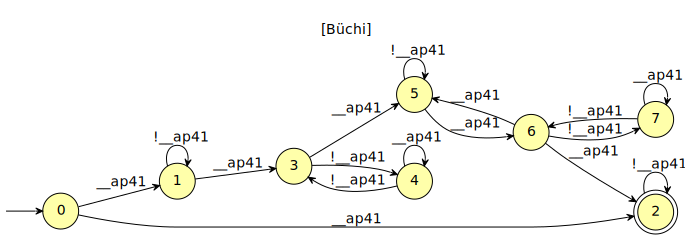
\includegraphics[width=0.7\textwidth]{images/unbordered_1_mod_6.pdf}
    \caption{A B\"uchi automaton accepting $(1|10^*1(01^*0)^*1(0^*(1(01^*0)^*1)^*11)0^{\omega}$ in least significant digit first representation.}
    \label{fig:unbordered_1_mod_6}
\end{figure}

\end{proof}

\section{Implementation}\label{sec:implementation}

This section describes at a high-level the implementation of Pecan.
First, we describe the syntax in Section~\ref{sec:ir-syntax}.
Then, we give a formal definition of the Pecan language, starting with the typing rules and associated definitions in Section~\ref{sec:typing}, and then the rules for evaluation in Section~\ref{sec:evaluation}.
Next, we describe each step of the AST to IR conversion in Section~\ref{sec:ast-to-ir}, and finally the various optimizations performed by Pecan prior to execution in Section~\ref{sec:optimizations}.

The process of executing a program is roughly as follows:

\begin{enumerate}
    \item Parse the program into an AST (Abstract Syntax Tree).
    \item Transform the program's AST into a simplified IR  representation, rewriting constructs such as $\iff$ in terms of simpler ones, like $\land$, $\lor$, and $\lnot$.
    \item Load the standard library (if desired); loading the standard library requires going through all of the steps again, starting from step 1, but skipping this step.
    \item Then, for each definition or directive, perform the following steps:
        \begin{enumerate}
            \item Run the untyped optimizer, if enabled.
            \item Perform type inference.
            \item Perform a final IR lowering.
            \item Run the typed optimizer, if enabled.
            \item Interpret the final IR of the current top-level construct.
        \end{enumerate}
\end{enumerate}

\subsection{IR Syntax}\label{sec:ir-syntax}

Below is the IR Syntax for the Pecan language; the full syntax that Pecan supports is much larger, but the rest of it is ``simply'' syntactic sugar which is expanded as explained in Section~\ref{sec:ast-to-ir}.

\begin{tabular}{c c l}
     Prog & \bnfdef & Definition$^*$ \\
     Definition & \bnfdef & $P(x_1 : \tau_1, \ldots, x_n : \tau_n)$ := Pred \\
     & \bnfalt & Restrict $x_1,\ldots,x_n$ are $P(y_1,\ldots,y_m)$ \\
     Pred & \bnfdef & true \bnfalt false \bnfalt Pred $\lor$ Pred \bnfalt $\lnot$ Pred \bnfalt Pred $\land$ Pred \\
     & \bnfalt & $\exists x. $ Pred \bnfalt E $<$ E \bnfalt E $=$ E \bnfalt @A[Pred] \bnfalt $P$(E, E, \ldots, E) \bnfalt Aut($V, \mathcal{A}$) \\
     E & \bnfdef & E + E \bnfalt E - E \bnfalt $x$ \bnfalt $i$ \bnfalt $f$(E, E, \ldots, E) 
\end{tabular}

\subsection{Type Checking}\label{sec:typing}

A \term{type} in Pecan is represented by a B\"uchi automaton.
We say that $x : \tau$ when $x \in L(\tau)$, sometimes simply written, as an analogy to logical predicates, as $\tau(x)$.
Additionally, types may be \term{partially applied}, i.e., $\tau = P(x_1, \ldots, x_n)$, where $P$ is some B\"uchi automaton.
Then $y : \tau$ when $(x_1, \ldots, x_n, y) \in L(P)$; and $\tau(y)$ holds when $y : \tau$.
In the concrete syntax of Pecan, we write \pecaninline{y is tau} or \pecaninline{y} $\in$ \pecaninline{tau}; for one or more variables, we can write \pecaninline{x, y, z are tau} to mean $x : \tau$, $y : \tau$, $z : \tau$.
Finally, there is a special type called $\inferred$, which should be thought of as a type that will be discovered later by how the value is used; or, as its name suggests, the type will eventually be \textbf{inferred} from context.
$L(\inferred)$ is undefined---$\inferred$ is NOT represented by an automata.

The judgement $\Gamma \proves x : \tau$ means that we can prove $\tau(x)$ is true in the environment $\Gamma$, which is a set of assumptions $x : \tau$.
The set $\{ x : \exists \tau. x : \tau \in \Gamma\}$ is the \term{domain} of $\Gamma$, written $\dom{\Gamma}$.
If for every $x \in \dom{\Gamma}$, there is a unique type $\tau$ such that $x : \tau \in \Gamma$, we say that $\Gamma$ is well-formed.
We assume that all contexts are well-formed unless otherwise specified.
The judgement $\Gamma \proves \prop{P}$ means that $P$ is a well-formed proposition in the environment $\Gamma$.
A predicate $P(\overline{x : \tau}) := Q$ is well-formed when $\overline{x : \tau} \proves \prop{Q}$.

We typecheck a sequence of Pecan predicates in order, starting with an empty environemnt $\Gamma = \emptyset$.
Below, we assume that the set of all well-formed predicates, which have already been checked, is ambiently available as $\mathcal{P}$.
Similarly, whenever we encounter a restriction, Restrict $x_1, \ldots, x_n$ are $P(y_1, \ldots, y_m)$, we update the current environment $\Gamma$ to be $\Gamma ~\cup~ \{ x_1 : P(y_1, \ldots, y_m), \ldots, x_n : P(y_1, \ldots, y_m, x_n) \} $; it is only allowed to use $P \in \mathcal{P}$, that is, predicates which have already been confirmed are well-formed.

\paragraph{Structures}

In order to provide a mechanism for ad-hoc polymorphism, Pecan allows the definition and use of \term{structures}.
This feature also facilitates the use of nicer syntax for arithmetic expressions (e.g., $x + (y + z) = w$ instead of $\exists t. \texttt{adder}(x, y, t) \land \texttt{adder}(t, z, w)$) without tying ourselves to a single numeration system.
For example, $\texttt{adder}$ will be resolved to some concrete predicate predicate based on the type of $x$, $y$, and $z$.
The exact rules and definitions related to this feature are given below.
We assume that structure definitions are ambiently available throughout the program.

\begin{definition}
    A \term{structure} is a pair $(t(x_1, \ldots, x_n), D)$ where each $x_i$ is an identifier, such that for some $\tau_1, \ldots, \tau_n$, $x_1 : \tau_1, \ldots, x_n : \tau_n \proves \prop{t(x_1, \ldots, x_n)}$ and $D$ is a map of identifiers to \term{call templates}; that is, it is of the form $f(y_1, \ldots, y_m)$, where each $y_i$ may be either: 1) $x_j$ for some $j$ or 2) $*$, which is pronounced ``any.''
    
    The \term{name} of the structure is $t$.
\end{definition}

We write the sequence of indexes of the arguments that are $*$, called \term{parameters}, as $\params(f(y_1, \ldots, y_m))$.
A call template is called $n$-ary if $|\params(f(y_1, \ldots, y_m))| = n$.
The sequence of the indexes of the other arguments, which are not $*$, called \term{implicits}, is written $\implicits(f(y_1, \ldots, y_m))$.
For example, $\params(f(a, *, *, b, *, *)) = [2, 3, 5, 6]$ and $\implicits(f(a, *, *, b, *, *)) = [1, 4]$.
We write $\params(f(y_1, \ldots, y_m))[i]$ (resp. $\implicits(f(y_1, \ldots, y_m))[i]$) to denote the $i$-th parameter (resp. implicit).

We assume that typechecking has been done before evaluating, because we may need structure information at run-time to resolve \term{dynamic calls}, that is, predicate calls whose name matches some definition inside a type.
We denote the type that an expression $e$ got when typechecking by $\typ{e}$.

We write $t[P] = Q(y_1, \ldots, y_m)$ to look up a definition in the associated map $D$, and we say that $t$ \term{has a definition} for $P$ in this case.
If $t$ does not have a definition for $P$, then we write $t[P] = \bot$.

\begin{definition}
    A structure is called \term{numeric} if it has a ternary definition for $\texttt{adder}$ and a binary definition $\texttt{less}$.
    We write $x + y = z$ when $\texttt{adder}(x, y, z)$ holds and $x < y$ when $\texttt{less}(x, y)$ holds.
    
    A numeric structure may also optionally contain the following definitions; otherwise a default predicate applies.
    
    \begin{itemize}
        \item[] A binary definition $\texttt{equal}$, written $x \equiv y$. 
            If not provided, the default is simply standard equality, $x = y$.
        
        \item[] A unary definition $\texttt{zero}$.
            If not provided, the default is $0^{\omega}$.
            
        \item[] A unary definition $\texttt{one}$.
            If not provided, the default is $x$ such that $0 \leq x \land \forall y. y = 0 \lor x \leq y$.
    \end{itemize}
\end{definition}

\begin{definition}
    The \emph{predecessor} of two types $\tau$ and $\sigma$, written $\tau \join \sigma$ is given by following partial function:
    \[
        \tau \join \sigma = 
        \begin{cases}
            \sigma & \tif \tau = \inferred~\text{and $\sigma$ is numeric} \\
            \sigma & \tif \forall \Free(\tau). \forall x. \tau(x) \implies \sigma(x) \\
            \tau & \tif \forall \Free(\tau). \forall x. \sigma(x) \implies \tau(x) \\
            \tau & \tif \sigma = \inferred~\text{and $\tau$ is numeric} \\
        \end{cases}
    \]
\end{definition}

\begin{definition}
    We can \term{resolve} a call $P(e_1, \ldots, e_n)$ as $Q(a_1 : \tau_1, \ldots, a_m : \tau_m)$, written $P(e_1, \ldots, e_n) \leadsto Q(a_1 : \tau_1, \ldots, a_m : \tau_m)$, if $Q(a_1 : \tau_1, \ldots, a_m : \tau_m) \in \mathcal{P}$ and for some structure $t(x_1, \ldots, x_\ell)$, for each $1 \leq i \leq n$, either:
    \begin{enumerate}
        \item $\typ{e_i} = t(x_1, \ldots, x_\ell)$, and $t[P] = Q(b_1, \ldots, b_m)$ such that
        for each $1 \leq j \leq m$,
        \[
            a_j =
            \begin{cases}
                x_k & \tif \implicits(Q(b_1, \ldots, b_m))[k] = j \\
                e_k & \tif \params(Q(b_1, \ldots, b_m))[k] = j
            \end{cases}
        \]
        
        \item $\typ{e_i} = s(y_1, \ldots, y_p)$, where $s \neq t$ and $s[P] = \bot$.
    \end{enumerate}
    
    or, if none of the arguments have a definition for $P$, then $P(e_1, \ldots, e_n) \leadsto P(a_1 : \tau_1, \ldots, a_m : \tau_m) \in \mathcal{P}$.
\end{definition}

\framebox{$\Gamma \proves e : \tau$} \textbf{Typing}
\begin{mathpar}
\inferrule*[right=Int]{
    i \in \Z
} { \Gamma \proves i : \inferred }

\inferrule*[right=Var]{
    x : \tau \in \Gamma
} { \Gamma \proves x : \tau }

% \reed{Not sure that I really want to support full type inference like this}
% \inferrule*[right=Var-Env]{
%     x \not\in \dom{\Gamma}
% }{ \Gamma \proves x : \inferred }

\inferrule*[right=Op]{ 
    \Gamma \proves a : \tau
    \and 
    \Gamma \proves b : \sigma
}{ \Gamma \proves a \oplus b : \tau \join \sigma }
\twhere \oplus \in \{ +, -, / \}

\inferrule*[right=Func]{
    \forall i \in \{ 1, \ldots, n \}. \Gamma \proves e_i : \tau_i
    \and
    f(x_1 : \tau_1, \ldots, x_n : \tau_n, r : \tau) \in \mathcal{P}
}{ \Gamma \proves f(e_1, \ldots, e_n) : \tau }
    
\end{mathpar}

\framebox{$\Gamma \proves \prop{P}$} \textbf{Well-formed Propositions}
\begin{mathpar}
\inferrule*[right=Rel]{ 
    \Gamma \proves a : \tau
    \and 
    \Gamma \proves b : \sigma
    \and
    \tau \join \sigma \neq \inferred
}{ \Gamma \proves \prop{a \Join b} }
\twhere \Join \in \{ \equiv, < \}

\inferrule*[right=BinPred]{
    \Gamma \proves \prop{P}
    \and
    \Gamma \proves \prop{Q}
}{ \Gamma \proves \prop{P \oplus Q} }
\twhere \oplus \in \{ \lor, \land \}

\inferrule*[right=Comp]{
    \Gamma \proves \prop{P}
}{ \Gamma \proves \prop{\lnot P} }

\inferrule*[right=Exists]{
    \Gamma, x : \tau \proves \prop{P}
}{ \Gamma \proves \exists x : \tau. \prop{P} }

\inferrule*[right=Call]{
    \forall i \in \{1, \ldots, n\}. \Gamma \proves e_i : \tau_i
    \and
    f(x_1 : \tau_1, \ldots, x_n : \tau_n) \in \mathcal{P}
}{ \Gamma \proves \prop{f(e_1, \ldots, e_n)} }

\inferrule*[right=Annotation]{
    \Gamma \proves \prop{P} 
}{ \Gamma \proves \prop{@A[P]} }

\inferrule*[right=Automaton]{
}{ \Gamma \proves \prop{\text{Aut}(V, \mathcal{A})} }
\end{mathpar}

\reed{TODO: Some proofs maybe (e.g., if $\Gamma \proves x : \tau$, then if $\Gamma$, then $x \in L(\tau)$, or if $\Gamma \proves \prop{P}$ then $P \evaluates \mathfrak{A}$ for some $\mathfrak{A}$}

\subsection{Evaluation}\label{sec:evaluation}

The Pecan interpreter is a simple tree-walking interpreter which typechecks, then processes, each top-level construct (see Section~\ref{sec:ir-syntax}) in sequential order.

Operations with non-trivial implementations are described in detail below.
Most basic automata operations (e.g., conjunction, disjunction, complementation, emptiness checking, simplification) are implemented using the Spot library \cite{duret.16.atva2}, so details of these algorithms are not presented here.

\subsubsection{Automata Representation}

Automata are represented by a pair of $(V, \mathcal{A})$, where $V$ is a map taking variable names to an ordered list of APs that represent it, called the \emph{variable map}, and $\mathcal{A}$ is a Spot automaton (specifically, a value of type \texttt{spot.twa\_graph}).
For more information about the underlying representation of Spot automata, see the Spot library \cite{duret.16.atva2}.
We use the convention that calligraphic letters represent actual B\"uchi automata, and Fraktur letters represent automata in the Pecan sense of a pair of a variable map and B\"uchi automaton.

\paragraph{Variable Maps}
A \emph{variable map} $V$ is a finite set of mappings $x \mapsto [\texttt{ap}_1, \ldots, \texttt{ap}_n]$ such that for all distinct variables $x$ and $y$, $V[x] \cap V[y] = []$.

We denote by $V[x]$ the list of APs that $x$ is represented by, and we denote by $V \cup W$ the union of two variables maps union, which is only defined when the only keys that $V$ and $W$ have in common have identical APs.
$V \sqcup W$ is the disjoint union of these maps.
$V \setminus K$ is the variable map containing every entry $x \mapsto a \in V$ such that $x \not\in K$.

For two variable maps $V$ and $W$, $V \ll W$ denotes their \emph{biased merge}, which is a pair $(U, \theta)$ of a variable map $U$ and a substitution $\theta$ such that $U = V \cup W\theta$.
A substitution is a set of mappings $a \mapsto b$ where $a$ and $b$ are both APs, which can be applied to a variable map or an automaton to rename the APs in them.
For example, if $\theta = \{ a \mapsto d, c \mapsto e \}$, then $\{ x \mapsto [ a, b, c ] \} \theta = \{ x \mapsto [ d, b, e ] \}$.
When it is clear, we also write $V \ll W$ to denote just the resulting variable map, without the associated substitution.

\subsubsection{Logical Operations}

Fundamental automata operations (i.e., $\land$ and $\lor$, represented by $\oplus$ below) are defined below.
\[
    (V, \mathcal{A}) \oplus (W, \mathcal{B}) = 
    \begin{cases}
        (V \ll W, \mathcal{A} \oplus \mathcal{B}) & \tif |S(\mathcal{A})| < |S(\mathcal{B})| \\
        (W \ll V, \mathcal{A} \oplus \mathcal{B}) & \owise
    \end{cases}
\]

where $S(\mathcal{A})$ denotes the set of states of $\mathcal{A}$.
For complements, we define $\lnot (V, \mathcal{A}) = (V, \lnot \mathcal{A})$.

Finally, automata literals, written Aut($V, \mathcal{A}$) simply evaluate to be the automata they store:
\begin{mathpar}

\inferrule*[right=Automaton]{
}{ \text{Aut}(V, \mathcal{A}) \evaluates (V, \mathcal{A}) }

\end{mathpar}

\subsubsection{Predicate Calls}

\begin{mathpar}
\inferrule*[right=Call]{
    \forall i. e_i \evaluates (\mathfrak{A}_i, x_i)
    \and
    \nonvar(e_1, \ldots, e_n) = [k_1, \ldots, k_{\ell}]
    \\
    P(x_1, \ldots, x_n) \leadsto Q(y_1, \ldots y_m)
    \and
    Q(z_1, \ldots, z_m) := R
    \and
    R \evaluates \mathfrak{B}
}{ P(e_1, \ldots, e_n) \evaluates \exists x_{k_1}, \ldots, x_{k_{\ell}}. \mathfrak{A}_1 \land \cdots \land \mathfrak{A}_n \land \mathfrak{B}[y_1 / z_1, \ldots, y_m / z_m] }
\end{mathpar}

where $\mathfrak{B}[y_1 / z_1, \ldots, y_m / z_m]$ denotes substituting each $y_j$ for $z_j$ in $\mathfrak{B}$, defined in Section~\ref{sec:impl-substitution}, and $\nonvar(e_1, \ldots, e_n)$ denotes the nonvariable positions in $e_1, \ldots, e_n$.

The rule for evaluating predicate calls is rather complicated, due to the possibility of dynamic calls.
Fundamentally, the rule does the following:

\begin{enumerate}
    \item Evaluates each argument $e_i$ as $(\mathfrak{A_i} x_i)$.
    \item Resolves the call $P$ as some predicate $Q$
    \item Evaluates the body of $Q$, $R$ and then substitutes in the variables $y_i$ (in the resolve call, some of which will be the result variables $x_i$) as appropriate.
    \item Projects out the intermediate result variables $x_{k_p}$, where the $k_p$ are the nonvariable positions in $e_1, \ldots, e_n$.
        This means that it only makes sense to use expressions whose output values will be well-behaved: that is, the resulting automaton should be the same regardless of which output was ``used.''
        Pecan will not automatically check this condition for performance reasons, but it is possible to do automatically.
\end{enumerate}

\subsubsection{Expressions}

Denote by $\Free(E)$ the list of free variables occurring in $E$.
For example, $\Free(a + b + c) = [a, b, c]$.
Denote by $E[v/x]$ the expression $E$ with $v$ substituted for $x$ where $x \in \Free(E)$.

An expression $E$ evaluates to a pair $(\mathfrak{A}, x)$ of an automaton $\mathfrak{A}$ and a variable $x$ where $\mathfrak{A}$ accepts $(v_1, \ldots, v_n, x)$ such that $\Free(E) = [x_1, \ldots, x_n]$ and $E[v_1/x_1, \ldots, v_n/x_n] = x$.

Note that many rules, like \textsc{Add} or \textsc{Equal} may need to evaluate subexpressions.
However, while evaluating a subexpression $e$, it may be that we generate fresh variables to store the result, which must be projected out.
The only case in which this does not occur is when the subexpression is itself a variable.

\begin{mathpar}
\inferrule*[right=Var]{ }{ x \evaluates (\top, x) }

\inferrule*[right=Add]{ 
    a \evaluates (\mathfrak{A}, x)
    \\
    b \evaluates (\mathfrak{B}, y)
    \\
    V = \{ v : (e, v) \in \{ (a,x), (b,y) \}, e \neq v \}
    \\
    (x + y = z) \evaluates \mathfrak{C}
} { a + b \evaluates (\proj_V(\mathfrak{A} \land \mathfrak{B} \land \mathfrak{C}), z) }
\twhere z ~ \text{is fresh}

\inferrule*[right=Sub]{ 
    a \evaluates (\mathfrak{A}, x)
    \\
    b \evaluates (\mathfrak{B}, y)
    \\
    V = \{ v : (e, v) \in \{ (a,x), (b,y) \}, e \neq v \}
    \\
    (z + y = x) \evaluates \mathfrak{C}
} { a - b \evaluates (\proj_V(\mathfrak{A} \land \mathfrak{B} \land \mathfrak{C}), z) }
\twhere z ~ \text{is fresh}

\inferrule*[right=Zero]{ }{ 0 \evaluates (\texttt{zero}(x), x) }
\twhere x ~ \text{is fresh}

\inferrule*[right=One]{ }{ 1 \evaluates (\texttt{one}(x), x) }
\twhere x ~ \text{is fresh}

\inferrule*[right=Int]{
    \overbrace{1 + 1 + \cdots + 1}^{n~\text{times}} \evaluates (\mathfrak{A}, x)
}{ n \evaluates (\mathfrak{A}, x) }
\twhere x ~ \text{is fresh}

\inferrule*[right=Func]{
    f(e_1, \ldots, e_n, x) \evaluates \mathfrak{A}
}{ f(e_1, \ldots, e_n) \evaluates (\mathfrak{A}, x) }
\twhere x ~ \text{is fresh}

\inferrule*[right=Equal]{ 
    a \evaluates (\mathfrak{A}, x)
    \and
    b \evaluates (\mathfrak{B}, y)
    \\
    V = \{ v : (e, v) \in \{ (a,x), (b,y) \}, e \neq v \}
    \\
    (x \equiv y) \evaluates \mathfrak{C}
} { a = b \evaluates \proj_V(\mathfrak{A} \land \mathfrak{B} \land \mathfrak{C}) }

\inferrule*[right=Less]{ 
    a \evaluates (\mathfrak{A}, x)
    \and
    b \evaluates (\mathfrak{B}, y)
    \\
    V = \{ v : (e, v) \in \{ (a,x), (b,y) \}, e \neq v \}
    \\
    (x < y) \evaluates \mathfrak{C}
} { a < b \evaluates \proj_V(\mathfrak{A} \land \mathfrak{B} \land \mathfrak{C}) }

\end{mathpar}

\subsubsection{Existential Quantification}

\begin{mathpar}
\inferrule*[right=Exist]{
    \tau(x) \land P \evaluates (V, \mathcal{A})
}{ \exists x \in \tau. P \evaluates (V \setminus \{x\}, \proj_x(\mathcal{A})) }
\end{mathpar}

Define $\proj_x(\mathfrak{A})$ to be $\proj_{\mathcal{V}[x]}(\mathcal{B})$, defined in the next section.

% \reed{Useless crossref atm, this is the next section...}
% For the actual implementation of the projection operation, see Section \ref{sec:impl-projection}.

\subsubsection{Projection}\label{sec:impl-projection}

Let $\mathfrak{A} = (Q, \Delta, \delta, q_0, F)$ be a B\"uchi automaton where $\Delta$ is the set of formulas involving $\land$, $\lor$, and $\lnot$ on a finite set $X$ of APs.
\reed{This is a nonstandard way to represent B\"uchi automata, but it's basically how Spot does it internally, and it's convenient for defining projection and substitution. I guess the alphabet is \emph{really} the set of equivalence classes of formulas modulo $\equiv$ such that $\varphi \equiv \psi$ if and only if $\varphi$ holds whenever $\psi$ does, but not sure that's necessary to write or interesting enough to include.}
We compute $\proj_Y(\mathcal{A}) = (Q, \Delta', \delta', q_0, F)$, where $Y$ is a finite list of APs and $\Delta'$ is the set of formulas on the APs $X \setminus Y$.
The new transition relation $\delta'$ is defined as
\[
    \delta' = \left\{ \left( s, d, \bigvee_{x \in Y} (\varphi[\top / x] \lor \varphi[\bot / x])  \right)  : (s, d, \varphi) \in \Delta' \right\}
\]
where $\varphi[a/x]$ is denotes $\varphi$ with $a$ substituted for $x$.
That is, for every transition from a state $s$ to a state $d$ on symbol $\varphi$, we have a transition from $s$ to $d$ whenever $\varphi$ holds regardless of whether any variable $x \in Y$ is true or false.

\subsubsection{Substitution}\label{sec:impl-substitution}

We define the substitution $\mathcal{A}[y/x]$, replacing $x$ by $y$ in the automaton $\mathcal{A} = (V, \mathcal{B})$ where $\mathcal{B} = (Q, \Delta, \delta, q_0, F)$ is a B\"uchi automaton as in Section~\ref{sec:impl-projection} with variables $X$ and underlying alphabet $\Sigma$.
Let $A = [a_1, \ldots, a_n]$ be the list of APs representing $x$ (i.e., $A = V[x]$), and let $B = [b_1, \ldots, b_n]$ be the list of APs representing $y$, which we assume is ambiently available.
This can be stored globally, and generated when needed if the variable $y$ has never been used before.
If $y$ has never been used before, we generate a new list of $n$ fresh APs.

Define $\mathcal{A}[y/x] := (V', \mathcal{B}')$ where $V' = (V \setminus \{ x \}) \cup \{ y \mapsto B \}$, and $\mathcal{B}' = (Q, \Delta', \delta', q_0, F)$, with the new set of variables $X' = (X \setminus A) \cup B$ and the same underlying alphabet, such that:
\[
    \Delta' = \{ \varphi[b_1/a_1, \ldots, b_n/a_n] : \varphi \in \Delta \}
\]
and
\[
    \delta' = \{ (s, d, \varphi[b_1/a_1, \ldots, b_n/a_n]) : (s, d, \varphi) \in \delta' \}
\]

\subsection{AST to IR Conversion}\label{sec:ast-to-ir}

The following conversions are performed when converting the AST to the IR:

\begin{itemize}
    \item $a \iff b$ becomes $(a \implies b) \land (b \implies a)$
    \item $a \implies b$ becomes $\lnot a \lor b$
    \item $k \cdot x$ becomes $\overbrace{x + \cdots + x}^{k \text{ times}}$
    \item $a \neq b$ becomes $\lnot (a = b)$
    \item $a > b$ becomes $b < a$
    \item $a \geq b$ becomes $b < a \lor a = b$
    \item $-a$ becomes $0 - a$
    \item $a \leq b$ becomes $a < b \lor a = b$
    \item $W[i] = W[j]$ becomes $W(i) \iff W(j)$
    \item $W[i] \neq W[j]$ becomes $\lnot (W[i] = W[j])$
    \item $W[i..j] = W[k..\ell]$ becomes $j + k = i + \ell \land \forall n \in \typ{i}. i + n < j \implies W[i + n] = W[k + n]$
    \item $W[i..j] \neq W[k..\ell]$ becomes $\lnot (W[i..j] = W[k..\ell])$
    \item $\forall x_1 \in \tau_1, \ldots, x_n \in \tau_n. P$ becomes $\lnot (\exists x_1 \in \tau_1, \ldots, x_n \in \tau_n. \lnot P)$
    \item $\exists x_1 \in \tau_1, \ldots, x_n \in \tau_n. P$ becomes $\exists x_1 \in \tau_1. \ldots. \exists x_n \in \tau_n. P$
\end{itemize}

where $\typ{i}$ denotes the type of $i$.

\section{Overview}\label{sec:features}

For full documentation on the features of Pecan, see the more comprehensive manual available at our repository~\cite{pecan-repo}.

% \paragraph{Functions}
% This is already shown in the implementation section, no need to discuss here
% Some predicates represent relations which are functions.
% For readability, Pecan allows the use of \term{placeholders}, which allow specifying the output of a function-like predicate.
% For example, if we have a predicate \pecaninline{bin\_add(x, y, z)} accepting triples such that $x + y = z$ for binary numbers $x$, $y$, and $z$, then \pecaninline{bin\_add(x, y, \_)} is equivalent to writing $x + y$.
% So we could have written \pecaninline{bin\_add(x, y, \_) = z} instead of \pecaninline{bin\_add(x, y, z)}.
% Such a formula will be translated into \pecaninline{existsv. bin_add(x, y, v) & v = z}.

% Because the last argument to a function-like relation is typically the output argument, we can simply write \pecaninline{f(x)} to mean \pecaninline{f(x, \_)}.

% \paragraph{Annotations}
% Pecan supports \term{annotations}, which may \term{wrapped} around any formula.
% They do \textbf{not} change the logical value of the automaton, but are instead used to tell Pecan how to evaluate a formula (e.g., when to simplify).
% The most commonly used annotations are:
% \begin{itemize}
%     \item \pecaninline{@postprocess[FORMULA]}: Performs a variety of simplification steps on the automaton representing \pecaninline{PREDICATE}.
%     \item \pecaninline{@no_simplify[FORMULA]}: Turns off simplification (on by default) for the formula and all its subformulas.
% \end{itemize}

\paragraph{Directives} are the interface to Pecan, instructing it to perform actions (e.g., prove a theorem).
We discuss the most important: \pecaninline{Restrict}, \pecaninline{Structure}, and \pecaninline{Theorem}.

\begin{pecan}
Restrict VARIABLES are TYPE_PREDICATE.
\end{pecan}

In all following code in the file in which the \pecaninline{Restrict} appears, the variables specified are now consider to be of the specified type.

\vspace{-0.5em}
\begin{pecan}
Structure TYPE_PREDICATE defining { FUNCTION_PREDICATES }
\end{pecan}
\vspace{-0.5em}

Defines a new structure.
The \pecaninline{TYPE_PREDICATE} is essentially the part written after the \pecaninline{is} in a restriction. 
For example, in \pecaninline{Restrict x is nat.}, the type predicate is \pecaninline{nat}; in \pecaninline{Restrict i is ostrowski(a).}, the type predicate is \pecaninline{ostrowski(a)}.
The function predicates become available to be called using the names in quotes---this feature allows for ad-hoc polymorphism, as described in Section~\ref{sec:implementation}.
It is also used to resolve arithmetic operators, such as \pecaninline{+} (which calls the relevant \pecaninline{adder}) and \pecaninline{<} (which calls the relevant \pecaninline{less}).

\vspace{-0.5em}
\begin{pecan}
Theorem ("THEOREM NAME", { PREDICATE }).
\end{pecan}
\vspace{-0.5em}
\pecaninline{Theorem} is the interface to the theorem proving capabilities of Pecan, stating that Pecan show attempt to prove the specified \pecaninline{PREDICATE} is true.

Below is an example of using all three features from above: specifying a structure called \pecaninline{nat}, restricting variables, and then proving a theorem, which is true because of the dynamic call resolution.
\vspace{-0.5em}
\begin{pecan}
Structure nat defining {
    "adder": bin_add(any, any, any),
    "less": bin_less(any, any)
}
Restrict a, b are nat.
Theorem ("", { forall a,b. a < b <=> bin_less(a,b)}).
\end{pecan}
\vspace{-0.5em}

\paragraph{Automatic Words}
Any predicate $P$ can be interpreted as a word by writing $P[i]$, which is treated as $1$ if $P(i)$ is true, and $0$ if $P(i)$ is false.
Currently only binary automatic words are supported.
We use the following translations into the IR:

\begin{itemize}
    \item $P[i] = 0 \leadsto \lnot P(i)$
    \item $P[i] = 1 \leadsto P(i)$
    \item $P[i] = Q[j] \leadsto P(i) \iff P(j)$
    \item $P[i] \neq Q[j] \leadsto \lnot (P(i) \iff P(j))$
    \item $P[i..j] = P[k..\ell] \leadsto j + k = i + \ell \land \forall n \in \typ{i}. i + n < j \Rightarrow P[i + n] = P[k + n]$
\end{itemize}

% \paragraph{Praline} is a functional language for metaprogramming that is a part of the Pecan system.
% We omit a full description due to space reasons, as it plays only a supporting role to the main system. 
% Some examples of its uses are:
% \begin{itemize}
%     \item Building automata that cannot be specified by a first-order formula involving other automata.
%     \item Defining useful helpers, such as \pecaninline{Theorem}, which generates certain Pecan definitions and statements.
% \begin{pecan}
% Define theoremCheck $\$$ID $\$$BODY := do
%   emit {$\$$ID() := $\$$BODY}; emit {#assert_prop(true,$\$$ID)}.
% Alias "Theorem" ==> Execute uncurry theoremCheck.
% Theorem ("Addition is commutative", 
% { forallx,y are nat. x + y = y + x }).
% \end{pecan}
%     \item Formatting the raw output of Pecan into human readable output.
%         For example, the real number encoding in Pecan represents $17/5$ as $00111(10000010)^\omega$.
%         Using Pecan, we can format this as $11.01(1001)^\omega$ in binary.
% \end{itemize}

% \begin{pecan}
% #save_aut(FILENAME, PREDICATE)
% #save_aut("bin_even.aut", bin_even)
% \end{pecan}

% Saves the predicate as an automaton in the modified HOA~\cite{hoa-format} format to the location specified.

% \begin{pecan}
% #load(FILENAME, FORMAT, PREDICATE)
% #load("bin_add.aut", "hoa", bin_add(a,b,c))
% #load("real/real_equal.txt", "pecan", real_equal(a, b))
% \end{pecan}

% Loads an automaton from a file with the specified name and arguments.
% Note that the number of arguments is \emph{NOT} checked for you.
% In general, you should be careful when loading automata from files because there are not many safeguards (it is assumed you know what you are doing).
% There are three currently supported formats: ``hoa''~\cite{hoa-format}, as described earlier; ``walnut'', the format that the automated theorem prover Walnut~\cite{walnut} uses; and ``pecan'', a custom format that Pecan uses, described below in the manual~\cite{pecan-repo}.

% \begin{pecan}
% #import(FILENAME)
% #import("integers.pn")
% \end{pecan}

% Loads all definitions from the specified file into the current scope.
% Does \emph{NOT} load restrictions into the current scope, but they function normally while evaluating the imported file.
% To control the search path, you can set the \lstinline{PECAN_PATH} environment variable.
% By default, the current working directory (at the time of loading the program), the directory the current source file is in, and the \lstinline{library/} directory of the Pecan directory.

\section{Case Study: Sturmian Words}\label{sec:sturmian-words}

One of the interesting applications of a theorem prover like Pecan is its ability to decide properties of automatic words, such as Sturmian words.
Not only can Pecan prove properties of such words, but it can also act as a (counter)example generator because of the constructive nature of its decision procedure: if property is \textbf{not} true, then Pecan can give a counterexample of exactly when it fails.
In this section, we explore several properties of Sturmian words using Pecan.

In Section~\ref{sec:sturmian-background} we give background definitions for words in general and then define Ostrowski numeration systems and Sturmian words.
In Section~\ref{sec:ostrowski-rep}, we describe the automata we created to decide properties of Sturmian words.
Finally, in Section~\ref{sec:sturmian-theorems}, we automatically prove many theorems about Sturmian words. \reed{some of which are new?}

\subsection{Background}\label{sec:sturmian-background}

\subsubsection{Ostrowski Numeration Systems}\label{sec:ostrowski-rep}
We write the \term{continued fraction} of a real number $x$ as a sequence of natural numbers  $x = [a_0,a_1,a_2,\ldots]$ such that 
\[
x = a_0+\cfrac{1}{a_1+\cfrac{1}{a_2+\cfrac{1}{a_3+\ddots}}}
\]

If the sequence is infinite and ultimately periodic with repeating part $a_i\dots a_j$, then we write this as $x = [a_0,a_1,a_2,\dots \overline{a_i,\dots,a_j}]$.

We make use of the \term{convergents} of the continued fraction to define an Ostrowski-$\alpha$ numeration system, where $\alpha$ is some positive irrational number.

\begin{equation*}
    \frac{p_n}{q_n} = [a_0, a_1, a_2, \ldots, a_n]
\end{equation*}

The sequences $p$ and $q$ are given by the following recursive definition.

\begin{equation}\label{eqn:conv-def}
\begin{split}
    p_{-2} = 0, \quad p_{-1} = 1, \quad p_n = a_n p_{n-1} + p_{n-2} \quad \text{for} \quad n \geq 0\\
    q_{-2} = 1, \quad q_{-1} = 0, \quad q_n = a_n q_{n-1} + q_{n-2} \quad \text{for} \quad n \geq 0
\end{split}
\end{equation}

% The convergents approximate $\alpha$, specifically:

% \begin{equation*}
%     \left| \alpha - \frac{p_n}{q_n} \right| < \frac{1}{q_n q_{n+1}} < \frac{1}{q_n^2} \quad \text{for all} \quad n.
% \end{equation*}

The \term{semiconvergent} sequences $p_{n,\ell}$ and $q_{n,\ell}$ are defined so that
\[
    \frac{p_{n,\ell}}{q_{n,\ell}} = \frac{\ell p_{n-1} + p_{n-2}}{\ell q_{n-2} + q_{n-2}}
\]
for $1 \leq \ell < a_n$.

Then every natural number $n$ may be written uniquely as a word $b_j b_{j-1} \cdots b_0$ where each $b_i \in \mathbb{N}$, such that $b_0 < a_0$, $b_i \leq a_i$, and if $b_i = a_i$, then $b_{i-1} = 0$~\cite{Ostrowski1922}.
That is, the following equation holds.

\begin{equation*}\label{eqn:ostrowski-def}
    n = \sum_{i=0}^j b_i q_i
\end{equation*}

We call this sequence $b_j b_{j-1} \cdots b_0$ the \term{canonical Ostrowski-$\alpha$ representation of $n$}, or simply the \term{Ostrowski-$\alpha$ representation $n$} when it is umabiguous.
We write the canonical Ostrowski-$\alpha$ representation of $n$ as $\mathcal{O}_{\alpha}(n)$.

For example, when $\alpha = \sqrt{2}$, the sequence $(q_n)$ starts out $1,2,5,12,\ldots$.
We can write $14_{10}$ in the Ostrowski-$\sqrt{2}$ numeration system as: $0\cdot1 + 1\cdot2 + 0\cdot5 + 1\cdot12$, or $1010_{\sqrt{2}}$.
Note there are two ways to write each number: least significant digit (LSD) and most significant digit MSD.
Above, $1010_{\sqrt{2}} = 14_{10}$ is written in the standard MSD form, however, our automata use LSD because it is more natural to create such automata for infinite strings, as they simply end in $0^\omega$ instead of having to add an additional symbol to the alphabet to indicate an end of number.

\subsubsection{Sturmian Words}

We now define \term{characteristic Sturmian words}.

Consider the standard coordinate plane, and some irrational number $\alpha \in (0,1)$.
Draw the line $y = \alpha x$.
We can define the \term{Sturmian words} via a \term{cutting sequence} given by this line in the standard coordinate plane; that is, as a sequence of letter corresponding to the grid lines crossed by the line.
We define the word $\text{cut}_{\alpha}$ as follows:
$\text{cut}_{\alpha}[n] = 0$ if the $n$-th line crossed by $y = \alpha x$ is a vertical line, and $\text{cut}_{\alpha}[n] = 1$ if it is a horizontal line.

Then the \term{characteristic Sturmian word with slope $\alpha$}, $C_{\alpha}$ is given by $C_{\alpha} = \text{cut}_{\alpha/(1-\alpha)}$~\autocite[Theorem 9.2.1]{auto_seq}.
Note that the first index of $C_{\alpha}$ is taken to be $1$, not $0$.
Using this procedure, we can see that $C_{\varphi}$, shown in Figure~\ref{fig:geom-sturmian-phi} starts out $10110101\ldots$.

\begin{figure}
    \centering
    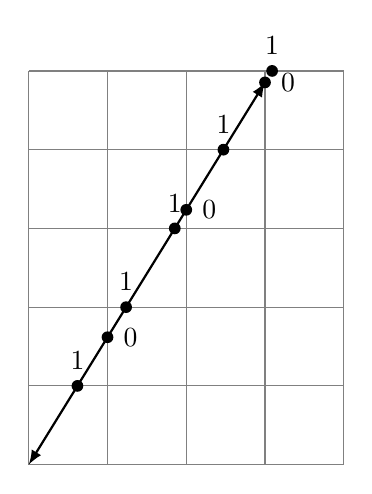
\begin{tikzpicture}
       \tkzInit[xmax=4,ymax=5,xmin=0,ymin=0]
       \tkzGrid
       \tkzAxeXY
       \draw[thick,latex-latex] (0,0) -- (3,3*1.61803) node[anchor=south west] {};
       
       \foreach \x in {1,2,3}{
            \node[fill=black, circle, inner sep=1.5pt, label=right:$0$] at (\x,\x*1.61803) {};
       }
       
       \foreach \y in {1,2,3,4,5}{
            \node[fill=black, circle, inner sep=1.5pt, label=above:$1$] at (\y/1.61803,\y) {};
       }
    \end{tikzpicture}
    \caption{The characteristic Sturmian word $C_{\varphi}$, defined by the cutting sequence $\text{cut}_{\varphi}$ with $\varphi = \frac{1 + \sqrt{5}}{2}$}
    \label{fig:geom-sturmian-phi}
\end{figure}

There is an intimate connection between the Ostrowski-$\alpha$ numeration system and the characteristic Sturmian word with slope $\alpha$, given by the following theorem (\autocite[Theorem 9.1.15]{auto_seq}).

\begin{theorem}\label{thm:ostrowski-sturmian}
Let $n \geq 1$ be an integer with Ostrowski-$\alpha$ representation: $b_j b_{j-1} \cdots b_0$.
Then $C_{\alpha}[n] = 1$ if and only if $b_j b_{j-1} \cdots b_0$ ends in an odd number of $0$'s.
\end{theorem}

In particular, this means that $C_{\alpha}$ is an automatic sequence, so we can create an automaton $\mathcal{C}_{\alpha}$ such that $\mathcal{C}(n)$ is true if and only if the $n$-th digit of $C_{\alpha}$ is $1$.
We define:
\[
    \mathcal{C}_{\alpha}[n] = 
    \begin{cases}
        1 & \tif C_{\alpha}(n) \\
        0 & \owise
    \end{cases}
\]

\subsubsection{Conventions}

Note that all quantifiers over Latin letters (e.g., $i, j, k, \ell, n, m$) are over the natural numbers, specifically over their Ostrowski-$\alpha$ representations.
When unclear from context which $\alpha$ is the base of the numeration system, we write $\N_{\alpha}$ to denote the Ostrowski-$\alpha$ representations of the natural numbers.
Quantifiers over the Greek letters (e.g., $\alpha$) are over the irrational numbers in $(0, 1)$, specifically over their continued fraction representations.
The real number and its continued fraction representation are used interchangably.
For example, when we say that $\alpha$ is eventually $1$, we mean that $\alpha = [a_1, a_2, \ldots, a_n, \overline{1}]$.

In all contexts below, unless otherwise noted, we use \term{Sturmian word} as a shorthand to refer to a \term{characteristic Sturmian word}.

\subsection{Representing Ostrowski Numeration Sytems}

In order to implement a decision procedure for Sturmian words, we need automata to recognize the following properties of Ostrowski-$\alpha$ numeration systems:

\reed{Maybe go into some more detail (e.g., that valid representations need to be of finite length).}

\begin{itemize}
    \item \pecaninline{bco_valid(a,x)}: If $x$ is a valid representation in the Ostrowski-$\alpha$ numeration system, given $\alpha$.
    We also define \pecaninline{ostrowski(x,a) :=  bco_valid(a,x)} for convenience.
    
    \item \pecaninline{bco\_leq(x,y)}: For two valid representations $x$ and $y$, if $x \leq y$.
    
    \item \pecaninline{bco\_adder(a,x,y,z)}: For three valid representations, $x$, $y$, and $z$, if $x + y = z$, given $\alpha$.
\end{itemize}

We encode representations of natural numbers in LSD in Ostrowski numeration systems using $\Sigma = \{0,1,2\}$ with each digit as a binary number in LSD and digits separated by $2$.
The encoding is the same for the slope $\alpha$, but note that because $\alpha \in (0, 1)$, we always have $\alpha = [0,a_1,a_2,\ldots]$, and so we omit the first coefficient, $0$, in our automata.
So an automaton accepting $([1][2])^{\omega}$ means that $\alpha = [0,\overline{1,2}]$.
Note that the continued fraction coefficients are unbounded, and so may be larger than $9$.
This matters because the string $8912$ could mean $[8,9,1,2]$, $[8,9,12]$, or $[8912]$, etc., so we write $[8][9][12]$ as appropriate to clarify what the string represents; however, the square brackets are \textbf{not} part of the language.
Finally, note that the second property can be decided without the parameter $\alpha$, but the first and third require it.

It is easy to encode the first two properties, but encoding a general addition automaton for Ostrowski numeration systems is more difficult. 

To see how we may construct an automaton to recognize Ostrowski addition for general continued fraction coefficients, we first define the vector space $\mathbb{Q}^\omega_{fin} = \oplus_{i < \omega} \mathbb{Q}$, i.e. the direct sum of $\omega$ many copies of $\mathbb{Q}$. This can also be constructed (with appropriate addition and multiplication) as a quotient of the language $\mathbb{Q}^*$ under the action of adding or removing a leading zero, so we will identify the vector space with $\mathbb{Q}^*$ for simplicity. Then the map:

$$v_\alpha : \mathbb{Q}^* \to \mathbb{R}, b_j b_{j-1} \dots b_0 \mapsto \sum_{i=0}^j b_i q_i$$

is linear, i.e. a homomorphism of $\mathbb{Q}$-vector spaces. Therefore, $\ker v_\alpha$, the set of Ostrowski-$\alpha$ representations of zero (with \textit{rational} coefficients), is itself a $\mathbb{Q}$-vector space. This vector space has a basis, which we call the \textit{carry basis,} consisting of all strings of the form $1(-a_i)(-1)0^{i-2}$ as well as the string $1(-a_1)$. It is elementary to check that this is a basis; one need only verify that

\begin{itemize}
	\item these vectors are all in $\ker v_\alpha$;
	\item they are all linearly independent, as they have different \textit{supports,} i.e. different indices of nonzero coefficients;
	\item by induction, we can add and subtract copies of these vectors from any initial string in $\ker v_\alpha$ in order to reduce it to a string of length $1$, which must be $0$.
\end{itemize}

Now in order to recognize whether the sum of two numbers with standard Ostrowski-$\alpha$ representations $(x_i)_i, (y_i)_i$ equals a number with standard Ostrowski-$\alpha$ representation $(z_i)_i$, after verifying that all three representations are standard, we need only check that $(x_i + y_i - z_i)_i$ is in $\ker v_\alpha$. In order to do this, we can use a division-like algorithm, subtracting multiples of the carry basis vectors from $(x_i + y_i - z_i)_i$ and checking if the last coefficient (the remainder) ends up being zero. Note that because the first coefficient in each carry basis vector is $1$, we will never need to use non-integer multiples of the carry basis vectors, so the entire algorithm can be carried out with all coefficients in $\mathbb{Z}$. In fact \christian{TODO: should we try to say / figure out why this is, or should we not bother?}, the only multiples of carry basis vectors that are necessary are $1$, $0$, and $-1$. So if none of those three coefficients properly zero out the current digit, we can immediately reject. This means that recognizing Ostrowski summation can be done with a finite automaton whose alphabet contains integers $\mathbb{Z}$ as follows:

\christian{TODO: Put Luke's automaton figure here. Do we have \TeX source for it?}

This automaton is uniform in $\alpha$ in the sense that it takes the continued fraction coefficients of $\alpha$ as additional input. Note then that each transition in this automaton, as well as the calculation of $x_i + y_i - z_i$, is an elementary calculation involving addition, subtraction, and constant numbers. Therefore, when given a numeric representation with finite alphabet wherein these operations are regular (in particular, binary representation), we can produce a finite automaton to recognize this relation where the strings $(a_i)_i, (x_i)_i, (y_i)_i, (z_i)_i$ are encoded using said representation. So this allows us to construct a finite automaton that takes as input these four strings, with each coefficient encoded in binary and delimiters between them, and recognizes whether the input is a valid sum in Ostrowski-$\alpha$ representation.
	
\reed{Note: the original automaton was in MSD, but we converted it to LSD.}

% \eric{Attempt} Luke Schaeffer
% \eric{We either cite from Luke or write it ourselves. If we were to write it ourself, then}
% \eric{Sketch:
% \begin{enumerate}
%     \item 0-space vector space
%     \item Carry base representation
%     \item  Coefficients are $\{-1,0,1\}$
%     \item  The first automaton with infinite alphabet has finite number of states (at most 10, one garbage, 9 labeled $\{-1,0,1\}\times \{-1,0,1\}$)
%     \item  We can transform the infinite alphabet into binary one. 
% \end{enumerate}

% }
% \eric{We do have enough information about how it works but maybe better}


\subsubsection{Derived Predicates}

Using the basic definitions above, we can encode the following useful predicates.

\begin{itemize}
    \item \pecaninline{bco\_zero(x)}: Checking whether $x$ is the representation of $0$, defined as $z$ such that $\forall y. z \leq y$.
    
    \item \pecaninline{bco\_eq(x,y)}: Checking whether $x = y$, defined as $x \leq y \land y \leq x$.
    
    \item \pecaninline{bco\_succ(a,x,y)}: The \term{successor} of $x$ (i.e., $x + 1$), defined as the number $y$ such that $x < y$ and $\forall z. z \leq x \lor y \leq z$.
\end{itemize}

\subsubsection{Proofs of Correctness}

Using Pecan, we can prove that the automata we have created are correct in a number of ways, by checking basic properties of addition and the natural numbers.

Because we have defined the successor of $x$ without reference to the addition automaton, we can use it to check the correctness of addition.
We check that our addition automaton conforms to the standard definition of addition on the natural numbers:
\begin{align*}
    0 + y &= y \\
    s(x) + y &= s(x + y)
\end{align*}

where $s(a)$ denotes the successor of $a$.
We check that our adder satisfies this property using the following Pecan code:

\begin{pecan}
Restrict x,y,z are ostrowski(a).
Theorem ("Addition base case.", {
    foralla. forallx,y,z. 
    if bco_zero(x) then 
        (bco_adder(a, x, y, z) <=> bco_eq(y, z))
}).

Theorem ("Addition inductive case.", {
    foralla. forallx,y,z,u,v. 
    if (bco_succ(a,u,x) & bco_succ(a,v,z)) then 
        (bco_adder(a,x,y,z) <=> bco_adder(a,u,y,v))
}).
\end{pecan}

We also verify that every natural number has a unique successor in each Ostrowski-$\alpha$ numeration system, and every natural number (apart from $0$) have a predecessor, where the predecessor of $y$ is $x$ such that \pecaninline{bco_succ(a,x,y)} holds.
We also prove some properties about the relationship between \pecaninline{bco_leq} and \pecaninline{bco_adder}.
\begin{pecan}
Theorem ("Every valid Ostrowski-a representation has a successor.", {
    foralla,x. if bco_valid(a,x) then existsu. bco_succ(a,x,u)
}).

Theorem ("All natural numbers other than 0 have a predecessor.", {
    forall a, x. 
    if bco_valid(a,x) then 
        (bco_zero(x) | (exists u. bco_succ(a,u,x)))
}).

Theorem ("For all x, y, and z, we have x <= y iff x + z <= y + z", {
    forall a. forall x,y,z,u,v. 
    if (bco_valid3(a,x,y,z) & bco_valid2(a,u,v) & bco_adder(a,x,z,u) & bco_adder(a,y,z,v)) then
        (bco_leq(x, y) <=> bco_leq(u, v))
}).

Theorem ("If x <= y, then there is some z so that x + z = y.", {
    forall a. forall x,y. 
    if bco_valid2(a,x,y) then 
        (bco_leq(x,y) <=> exists z. bco_adder(a,x,z,y))
}).
\end{pecan}

There are many other simple correctness properties we check, such as $\leq$ being a total order, which can be found in our project repository at \url{https://github.com/ReedOei/SturmianWords}.

\subsection{Results}\label{sec:sturmian-theorems}

\reed{Report performance statistics and automaton sizes probably}

In this section we use Pecan to prove many theorems about Sturmian words.

Because comparing factors of Sturmian words is so widely useful, we create an automaton called $\texttt{factor\_lt}(\alpha, i,j,k)$ which holds if and only if $C_{\alpha}[i..j] = C_{\alpha}[k..\ell]$ where $\ell = j - i + k$ and $i \leq k$.
This last restriction reduces the size of the automaton Pecan must complement to construct \texttt{factor\_lt}, improving performance, and in most cases it poses no problems.
In the cases that we truly need to remove the restriction, we can simply write the \term{bidirectional} version: $\texttt{factor\_lt}(\alpha,i,j,k) \lor \texttt{factor\_lt}(\alpha,k,\ell,i)$ where $\ell = j - i + k$.
Throughout this paper, we write $C_{\alpha}[i..j] = C_{\alpha}[k..\ell]$ to mean $\texttt{factor\_lt}(\alpha,i,j,k)$ or the bidirectional version (whichever is appropriate for the situation) for readability reasons.
Note that the exact predicates and many of the intermediate automata are available in the following GitHub repository: \url{https://github.com/ReedOei/SturmianWords}.

As the automata tend to be large, almost all having 100 or more states and hundreds of edges, displaying them graphically provides little insight, and so we omit such diagrams below.

\subsubsection{Periodicity}

We begin with a well-known result about Sturmian words: that they are not eventually periodic.
In fact, a binary $\omega$-word is a Sturmian word if and only if it is a balanced, aperiodic binary word (\autocite[Theorem 2.1.5]{zbMATH01737190}).

\begin{definition}
    An $\omega$-word $w$ is \term{eventually periodic with period $p$} for some $p > 0$ if there is some natural number $n$ so that $w[i] = w[i + p]$ for all $i > n$.
\end{definition}

\begin{theorem}
No Sturmian word is eventually periodic.
\end{theorem}
\begin{proof}
Using Pecan, we construct an automaton recognizing the following property:
\[
    \texttt{eventually\_periodic}(\alpha, p) := p > 0 \land \exists n. \forall i > n. C_{\alpha}[i] = C_{\alpha}[i + p]
\]

In Pecan, this can be written as:

\begin{pecan}
Restrict a is bco_standard.
Restrict i, n, p are ostrowski(a).
eventually_periodic(a, p) := 
    p > 0 & existsn. foralli. if i > n then $\$$C[i] = $\$$C[i + p]
\end{pecan}

The resulting automaton has $4941$ states and $35776$ edges, and takes \pecaninline{117.78} seconds to build.
Finally, we use Pecan to construct the automaton recognizing the following, which takes \pecaninline{35.3} seconds.
\[
    \forall \alpha, p. \lnot \texttt{eventually\_periodic}(\alpha, p)
\]

In Pecan, we write this statement as:

\begin{pecan}
Theorem ("Sturmian words are not eventually periodic", {
    foralla, p. if p > 0 then !eventually_periodic(a, p)
}) .
\end{pecan}

The resulting automaton is the $\top$-automaton, which proves the theorem.
\end{proof}

In the rest of this paper, we omit the exact input given to Pecan, and instead write the property definitions in a more typical style for readability.
Please refer to the repository linked above for the exact inputs.

\subsubsection{Powers}

\reed{Find other papers which prove these same theorems to cite.}

Next, we prove the follow results about \term{powers} of Sturmian words.

\begin{definition}
    A finite subword $x$ of a (finite or $\omega$) word $w$ is a \term{$n$-th power} if $x = y^n$ for some finite word $y$.
    We call a $2$nd power a \term{square}, and a $3$rd power a \term{cube}.
    
    A word that does not contain $n$-th powers is called \term{$n$-th power free} (or \term{square-free}, \term{cube-free} when appropriate).
\end{definition}

\begin{theorem}
    Sturmian words contain squares.
\end{theorem}
\begin{proof}
Using Pecan, we construct an automaton recognizing the following property, stating that there is a square of length $n$ starting at $C_{\alpha}[i]$.
\[
    \texttt{square}(\alpha, i, n) := n > 0 \land i > 0 \land \forall j. i \leq j < i + n. C_{\alpha}[j] = C_{\alpha}[j + n]
\]

The resulting automaton has 80 states and 400 edges.
Finally, Pecan proves the following in \pecaninline{0.02} seconds.
\[
    \forall \alpha. \exists i, n. \texttt{square}(\alpha, i, n)
\]
\end{proof}

In fact, all sufficiently long (i.e., longer than $4$ letters) binary words contain squares.
However, it is still useful to have create an automaton for recognizing squares, because it encodes quite a bit more information than just that squares exist: it also tells us exactly where they are in the Sturmian word.
Furthermore, we can use an automaton recognizing squares to efficiently build automata recognizing higher-powers.
We now reprove the following theorem from \autocite[Proposition 4.1]{PELTOMAKI2015886} and \autocite[Theorem 1]{DAMANIK2003377}.
\begin{theorem}
    If $n$ is the order of a power in $C_{\alpha}$, then $n = q_{n,\ell}$ for some $n$ and $\ell$; that is, $n$ is the denominator of a semiconvergent of $\alpha$.
\end{theorem}
\begin{proof}
    First, note that if $n$ is the denominator of a semiconvergent of $\alpha$, then its Ostrowski-$\alpha$ representation is of the form $0^*1b$ for some digit $b$ (which may be zero).
    We easily manually construct an automaton accepting such representations, called $\texttt{semiconvergent}$.
    Note that we only need to prove the theorem for squares, because any higher power starts with a square.
    
    We now use Pecan to prove the following statement is true
    \[
        \forall \alpha, i > 0, n > 0. \texttt{square}(a,i,n) \implies \texttt{semiconvergent}(n)
    \]
    Pecan proves the theorem in \pecaninline{0.21} seconds.
\end{proof} 

Sturmian words have the interesting property that they start with arbitrarily long squares (\autocite[Theorem 1]{Dubickas2009}).

\begin{theorem}
    All Sturmian words start with arbitrarily long squares.
\end{theorem}
\begin{proof}
Using Pecan and the automaton for squares that we constructed earlier, we prove the following predicate is true, which takes \pecaninline{0.40} seconds.
\[
    \forall \alpha. \forall j. \forall n. \exists m > n. \texttt{square}(a, j, m)
\]
\end{proof}

The following two theorems are consequences of \autocite[Theorem 4]{DAMANIK2003377}, which we can prove using Pecan.
\reed{Maybe remove this theorem because it's a consequence of the next theorem about cubic prefixes and it's basically identical to the one for squares?}
\begin{theorem}
    All Sturmian words contain cubes.
\end{theorem}
\begin{proof}
We construct an automaton recognizing the following property, stating that there is a cube of length $n$ starting at $C_{\alpha}[i]$.

We can use the previously defined square to define cubes, as follows:
\[
    \texttt{cube}(\alpha, i, n) := \texttt{square}(\alpha, i, n) \land \texttt{square}(\alpha, i + n, n)
\]

Finally, Pecan proves the following in \pecaninline{0.25} seconds.
\[
    \forall \alpha. \exists i, n. \texttt{cube}(\alpha, i, n)
\]
\end{proof}

Similar to squares, we have the following property about cubic prefixes
\reed{citation? or new?}
\begin{theorem}
    A Sturmian word starts with arbitrarily long cubes if and only if its continued fraction is not eventually 1.
    \reed{Because pictures are nice, I could change this into a more picture-y proof (the automata should be quite small) by creating the picture of the automata accepting Sturmian words with arbitrarily long cubic prefixes. Do we want that?}
\end{theorem}
\begin{proof}
First, we manually build an automaton recognizing $\alpha$ such that the continued fraction of $\alpha$ is not eventually one, called $\texttt{eventually\_one}$.

Pecan proves the following in \pecaninline{2.37} seconds:
\[
    \forall \alpha. 
    (\lnot \texttt{eventually\_one}(\alpha)) 
    \iff 
    \forall n.
    \exists m > n. \texttt{cube}(a, 1, m)
\]
\end{proof}

\begin{theorem}
    If $\alpha \in (0,1)$ is not eventually one, then $C_{\alpha}$ contains a fourth power.
\end{theorem}
\begin{proof}
We construct an automaton recognizing the following property, stating that there is a fourth power of length $n$ starting at $C_{\alpha}[i]$.
We can use the previously defined square and cube definitions to define fourth powers, as follows:
\[
    \texttt{fourth\_pow}(\alpha, i, n) := \texttt{square}(\alpha, i, n) \land \texttt{cube}(\alpha, i + n, n)
\]

Finally, Pecan proves the following in \pecaninline{0.56} seconds.
\[
    \forall \alpha. \lnot \texttt{eventually\_one}(\alpha) \implies \exists i, n. \texttt{fourth\_pow}(\alpha, i, n)
\]
\end{proof}

The converse is not true, and using Pecan, we can easily see why not.
We can ask Pecan for counterexamples to the converse using the following commands.

\begin{pecan}
Restrict i, n are ostrowski(a).
has_fourth_pow(a) := existsi,n. n > 0 & fourth_pow(a,i,n)
Example (ostrowskiFormat, { 
    bco_standard(a) & eventually_one(a) & has_fourth_pow(a) 
}).
\end{pecan}

Pecan responds with:

\begin{pecan}
[(a,[6][3]([1])^$\omega$)]
\end{pecan}

Meaning that $\alpha = [0,6,3,\overline{1}]$ is a counterexample (recall that $\alpha \in (0,1)$, so the first digit of the continued fraction is always $0$); indeed, $C_{\alpha}$ starts as $000001\ldots$, so there is a fourth power immediately at the beginning of it.
Using a sufficiently high starting coefficient, $\alpha = [a_0, a_1, \ldots]$, we can get any power, because the representations for $x$ with $0 < x < a_0$ will all start with an even number of zeros, and so $C_{\alpha}[x] = 0$.

\subsubsection{Mirror Invariance}

It will be useful to define a \term{reverse factor}:
\[
    \texttt{reverse\_factor}(a, i, j, \ell) := 0 < i < j \land \ell > 0 \land \forall t. i \leq t < j \implies C_{\alpha}[t] = C_{\alpha}[\ell + i - t] 
\]
That is, $\texttt{reverse\_factor}(a, i, j, \ell)$ is true when $C_{\alpha}[i..j] = (C_{\alpha}[k + 1..\ell + 1])^R$, where $\ell - k = j - i$.
We omit $k$ from the definition, because it is not necessary and would only serve to make the automaton larger.

\begin{definition}
    A word $w$ is called \term{mirror-invariant} if for every factor $x$ of $w$, the word $x^R$ is also a factor of $w$.
\end{definition}

We now recover the following proposition (\autocite[Proposition 2.1.19]{zbMATH01737190}):
\begin{theorem}
    All Sturmian words are mirror-invariant.
\end{theorem}
\begin{proof}
    We first define that a single factor $C_{\alpha}[i..j]$ is mirror-invariant if it satisfies:
    \[
        \texttt{mirror\_invariant}(\alpha,i,j) := \exists \ell. \texttt{reverse\_factor}(a,i,j,\ell)
    \]
    This takes \pecaninline{1135.38} seconds (about \pecaninline{19} minutes), and has $520$ states and $4442$ edges.
    
    Then using Pecan, we prove the following theorem, which takes \pecaninline{16.6} seconds:
    \[
        \forall \alpha, i,j. 0 < i < j \implies \texttt{mirror\_invariant}(a,i,j)
    \]
\end{proof}

\subsubsection{Palindromes}

\begin{definition}
    A word $x$ is a palindrome if $x = x^R$.
\end{definition}

Using the reverse factor automaton, is it quite easy to define a palindrome:
\[
    \texttt{palindrome}(\alpha, i, n) := \texttt{reverse\_factor}(a, i, i + n, i + n - 1)
\]
The resulting automaton has $342$ states and $1982$ edges, and takes \reed{get this number} seconds to build.

\begin{theorem}
    All Sturmian words start with arbitrarily long palindromes.
\end{theorem}
\begin{proof}
Pecan confirms the following predicate is true in \pecaninline{11.11} seconds.
\[
    \forall \alpha. \forall m. \exists n. n > m \land \texttt{palindrome}(a, 1, n)
\]
\end{proof}

\begin{theorem}
    All Sturmian words contain palindromes of every length $n \geq 0$.
\end{theorem}
\begin{proof}
    Pecan confirms the following predicate is true in \pecaninline{2.40} seconds.
    \[
        \forall \alpha. \forall n > 0. \exists i. \texttt{palindrome}(a, i, n)
    \]
\end{proof}

\begin{theorem}
    Let $n$ be a natural number and $\alpha \in (0, 1)$ an irrational number.
    Then $C_{\alpha}$ contains exactly one palindrome of length $n$ if $n$ is even, and exactly two palindromes of length $n$ if $n$ is odd.
    \reed{This theorem also implies that $C_{\alpha}$ contains palindromes of every length, so the previous theorem is unnecessary}
\end{theorem}
\begin{proof}
    We begin by defining a predicate defining the location of the first occurrence of each length $n$ palindrome in $C_{\alpha}$.
    \[
        \texttt{first\_palindrome}(a,i,n) :=
            \texttt{palindrome}(a,i,n)
            \land
            \forall j > 0. C_{\alpha}[j..j+n] = C_{\alpha}[i..i+n] \implies i \leq j
    \]
    The resulting automaton has $247$ states and $1281$ edges.
    The following predicate is states the theorem, and Pecan proves it in \pecaninline{428.85} seconds (about 7 minutes).
    \begin{align*}
        \forall \alpha, n. & \\
            & (\texttt{even}(\alpha, n) \implies \exists i. \forall k. \texttt{first\_palindrome}(a,k,n) \iff i = k) \land \\
            & (\texttt{odd}(\alpha, n) \implies \exists i,j. i \neq j \land \forall k. \texttt{first\_palindrome}(a,k,n) \iff (i = k \lor j = k))
    \end{align*}
    We define even and odd in the standard way: $\texttt{even}(\alpha, n) := \exists m. n = 2m$ and we define $\texttt{odd}(\alpha, n) := \lnot \texttt{even}(\alpha, n)$.
\end{proof}

\reed{Something to note, perhaps, is that the fastest way to generate these automata is not always the predicate that is the most obvious (e.g., above, that way is much more efficient than the naive way of starting out with a definition based on the length of the factor}

\subsubsection{Antisquares and Antipalindromes}

Similar to squares and palindromes are the concepts of antisquares and antipalindromes, which share many of the same properties.
First, we define antisquares and antipalindromes.

\begin{definition}
    A word $w$ is an \term{antisquare} if it is of the form $w = x \overline{x}$ for some $x$.
    The \term{order} of $w$ is $|x|$.
\end{definition}

\begin{definition}
    A word $w$ is an \term{antipalindrome} if $w = \overline{w^R}$.
\end{definition}

Unlike squares and palindromes, of which all Sturmian words contain many distinct examples, there are both finitely many antisquares and antipalindromes in each Sturmian word.

\begin{theorem}
    All Sturmian words contain finitely many antisquares.
\end{theorem}
\begin{proof}
Similar to squares, we construct an automaton recognizing the following property that there is an antisquare of order $n$ at $C_{\alpha}[i..i+2*n]$.
\[
    \texttt{antisquare}(\alpha, i, n) := n > 0 \land i > 0 \land \forall j. i \leq j < i + n \implies C_{\alpha}[j] \ne C_{\alpha}[j + n]
\]

Finally, Pecan proves the following in \pecaninline{0.17} seconds.
\[
    \forall \alpha. \exists m. \forall n, i. \texttt{antisquare}(\alpha, i, n) \implies n < m
\]
\end{proof}

\begin{theorem}
    All Sturmian words contain finitely many antipalindromes.
\end{theorem}
\begin{proof}
    We construct the following definition of an antipalindrome, stating that $C_{\alpha}[i..j]$ is an antipalindrome:
    \[
        \texttt{anti\_palindrome}(\alpha, i, n) := 
            \forall t. i \leq t < i + n \implies C_{\alpha}[t] = C_{\alpha}[j + i - t]
    \]
    The resulting automaton has $168$ states and $591$ edges which takes \pecaninline{359.52} seconds to build (roughly \pecaninline{6} minutes).
    
    Pecan confirms the following predicate is true, proving the theorem, which takes \pecaninline{0.12} seconds to run.
    \[
        \forall \alpha. \exists m. \forall i, n. \texttt{anti\_palindrome}(\alpha, i, n) \implies n \leq m
    \]
\end{proof}

% We can bound the possible lengths of antisquares and antipalindromes using the continued fraction's convergents.
% We define $A_O : (0,1) \to \N$ such that $A_O(\alpha)$ is the maximum order of any antisquare in $C_{\alpha}$; we also define $A_L : (0,1) \to \N$ such that $A_L(\alpha)$ is the maximum length of any antisquare in $C_{\alpha}$.
% Note that $A_L(\alpha) = 2A_O(\alpha)$.

% Similarly, define $A_P : (0, 1) \to \N$ such that $A_P(\alpha)$ is the maximum length of any antipalindrome in $C_{\alpha}$.

% \begin{theorem}
%     For every $\alpha = [a_0, a_1, a_2, \ldots] \in (0,1)$, the following are true:
%     \begin{enumerate}[label=(\roman*)]
%         \item $A_O(\alpha) \leq a_3 q_3 + a_1 q_1$
%         \item $A_P(\alpha) \leq a_3 q_3 + a_1 q_1$ 
%         \item $A_L(\alpha) \leq a_5 q_5 + a_3 q_3 + a_1 q_1$
%         \item $A_O(\alpha) \leq A_P(\alpha) \leq A_L(\alpha) = 2A_O(\alpha)$
%     \end{enumerate}
    
%     That is, the longest antipalindrome in $C_{\alpha}$ is at least as long as the largest order of an antisquare in $C_{\alpha}$, but it is shorter than the longest antisquare.
%     Additionally, there are $\alpha, \beta \in (0, 1)$ for which the equality is achieved; that is, there is are $\alpha, \beta \in (0, 1)$ such that $A_O(\alpha) = A_P(\alpha)$ and $A_P(\beta) = A_L(\beta)$.
% \end{theorem}
% \begin{proof}
%     Using Pecan, we create automata which compute $A_O$, $A_P$, and $A_L$:
%     \begin{align*}
%         A_O(\alpha, n) &:= \texttt{has\_antisquare}(\alpha, n) \land \forall m. \texttt{has\_antisquare}(\alpha, m) \implies m \leq n \\
%         A_P(\alpha, n) &:= \texttt{has\_antipalindrome}(\alpha, n) \land \forall m. \texttt{has\_antipalindrome}(\alpha, m) \implies m \leq n \\
%         A_L(\alpha, n) &:= \texttt{has\_antisquare\_len}(\alpha, n) \land \forall m. \texttt{has\_antisquare\_len}(\alpha, m) \implies m \leq n
%     \end{align*}
%     % This is probably obvious
%     % where $\texttt{has\_antisquare}(a, n)$ holds when $C_{a}$ has an antisquare of order $n$, $\texttt{has\_palindrome}(a, n)$ holds when $C_{a}$ has an antipalindrome of length $n$, and $\texttt{has\_antisquare\_len}(a, n)$ holds when $C_{a}$ has an antisquare of length $n$.
%     We then verify some basic correctness properties:
%     \begin{itemize}
%         \item Each of these relations is a function, which justifies using Pecan's functional expression notation (e.g., $A_L(\alpha) = 2A_O(\alpha)$ instead of $A_L(\alpha, 2n) \land A_O(\alpha, n)$).
%         \item $A_L(\alpha) = 2A_O(\alpha)$
%         \item $A_O(\alpha) \geq 1$, $A_L(\alpha) \geq 2$, and $A_P(\alpha) \geq 2$; because every Sturmian word must contain $01$ which is both an antisquare and an antipalindrome.
%     \end{itemize}
    
%     We use Praline to build automata recognizing Ostrowski-$\alpha$ representations of at most $4$ and $6$ nonzero digits, called $\texttt{is\_4\_digits}(n)$ and $\texttt{is\_6\_digits}(n)$.
%     The we use Pecan to prove all the parts of the theorem:
%     \begin{align*}
%         \forall \alpha. & \texttt{is\_4\_digits}(A_O(\alpha)) \land \texttt{is\_4\_digits}(A_P(\alpha)) \land \texttt{is\_6\_digits}(A_L(\alpha)) \land \\
%                         & A_O(\alpha) \leq A_P(\alpha) \leq A_L(\alpha)
%     \end{align*}
%     We also use Pecan to find examples of the equality: when $\alpha = [0,3,3,\overline{1}]$, we have $A_O(\alpha) = A_P(\alpha) = 2$, and when $\alpha = [0,4,2,\overline{1}]$, we have $A_P(\alpha) = A_L(\alpha) = 2$.
    
%     The total time for the proof, including the correctness properties is \pecaninline{4.16} seconds.
    
%     Finally, for parts (1)-(3) of the theorem, note that we have proven:
%     \begin{enumerate}
%         \item $|\mathcal{O}_{\alpha}(A_O(\alpha))| \leq 4$
%         \item $|\mathcal{O}_{\alpha}(A_P(\alpha))| \leq 4$ 
%         \item $|\mathcal{O}_{\alpha}(A_L(\alpha))| \leq 6$
%     \end{enumerate}
%     But this implies that $A_O(\alpha) \leq a_3 q_3 + a_1 q_1$, and similarly for the others, because the largest length-$4$ Ostrowski-$\alpha$ representation is the representation of $a_3 q_3 + a_1 q_1$.
% \end{proof}

\subsubsection{Special Factors}

\begin{definition}
    A factor $x$ of a word $w$ is called \term{right special} (or just \term{special}) if $x0$ and $x1$ are both factors of $w$.
\end{definition}

\begin{theorem}
    The unique special factor of length $n$ is $C_{\alpha}[1..n+1]^R$.
\end{theorem}
\begin{proof}   
    We define \texttt{special} as:
    \[
        \texttt{special}(\alpha,i,n) := 
            (\exists j. C_{\alpha}[i..i+n] = C_{\alpha}[j..j+n] \land C_{\alpha}[j] = 0) \land
            (\exists k. C_{\alpha}[i..i+n] = C_{\alpha}[k..k+n] \land C_{\alpha}[k] = 1)
    \]
    Then we define \texttt{first\_special} as:
    \[
        \texttt{first\_special}(\alpha,i,n) := \texttt{special}(a,i,n) \land \forall j. C_{\alpha}[i..i+n] = C_{\alpha}[j..j+n] \implies i \leq j
    \]

    Pecan build this automaton in \pecaninline{91.99} seconds, has $112$ states and $447$ edges. 

    Recall that $\texttt{reverse\_factor}(\alpha,i,j,\ell)$ holds when $C_{\alpha}[i..j] = C_{\alpha}[k+1..\ell+1]^R$ where $k$ is such that $\ell - k = j - i$.
    Then we can state the theorem as:
    \[
        \forall \alpha, i > 0, n. \texttt{first\_special}(\alpha,i,n) \implies \texttt{reverse\_factor}(\alpha,i,i+n,n)
    \]
    
    Pecan proves this in \pecaninline{0.50} seconds.
\end{proof}

\subsubsection{Recurrent Factors}

\begin{definition}
    A factor $x$ of a word $w$ is called \term{recurrent} if it occurs infinitely often in $w$.
\end{definition}

\begin{theorem}
    For every $\alpha$, every factor of $C_{\alpha}$ is recurrent.
\end{theorem}
\begin{proof}
    We can easily define when a factor is recurrent.
    \reed{Finish this}
\end{proof}

% \subsubsection{Least Periods}

% \begin{theorem}\label{thm:least-period-semiconvergent}
%     If $p$ is the least period of a factor of $C_{\alpha}$, then $p$ is the denominator of a semiconvergent of $\alpha$; i.e., $p = q_{n,\ell}$ for some $n$ and $\ell$.
% \end{theorem}
% \begin{proof}
% \reed{least period takes 5016.77 seconds to build given the period automaton.}
% \end{proof}

\subsubsection{Unbordered Factors}

% \begin{definition}
%     A word $w$ is called \term{unbordered} if the least period of $w$ is $|w|$.
% \end{definition}

\reed{Still need to do the thing with the unbordered factors reversed/how many of them there are}

\reed{Maybe there's some relation between palindromes and unbordered factors because there's exactly two or each for each odd $n$ (or even i don't remember right now). Well, maybe not; palindromes are like, super bordered factors; unbordered factors are more like antipalindromes but somewhat less extreme. }

% We recover Lemma 8 of~\cite{Currie2009LeastPO}.
% \begin{theorem}
%     The least period of $C_{\alpha}[i..j]$ is the length of the longest unbordered factor of $C_{\alpha}[i..j]$.
% \end{theorem}
% \begin{proof}
% We have previously defined least periods, so we can easily define unbordered factors; similarly, it is straight to define unbordered subfactors:
% \begin{align*}
%     \texttt{unbordered}(\alpha,i,j) &:= \texttt{least\_period}(\alpha,j - i, i, j) \\
%     \texttt{unbordered\_factor}(\alpha,i,j,k,\ell) &:= i \leq j \land \ell \leq j \land \texttt{unbordered}(\alpha,k,\ell) 
% \end{align*}

% Then the theorem we wish to prove is
% \[
%     \forall \alpha. \forall i > 0, j > 0, p > 0.
%         \texttt{least\_period}(\alpha,p,i,j) \iff p = \max \{ m : \exists k. \texttt{unbordered\_factor}(\alpha,i,j,k,k+m)\}
% \]

% Pecan confirms the theorem is true.
% \end{proof}

% Note that from this theorem and Theorem~\ref{thm:least-period-semiconvergent}, it follows that the lengths of unbordered factors are also denominators of the semiconvergents of $\alpha$.

\section{Related Work}\label{sec:related-work}

\reed{talk about walnut here/anything esle relevant? probably mention the fibonacci word paper since we do so much of the same stuff}

\reed{might be worth talking about SPIN?}


\printbibliography

\appendix
\section{Automata Formats}\label{sec:aut-format}

Below are details on all the automata formats that Pecan supports.
Note that all formats support both deterministic and nondeterministic automata.

\subsection{HOA}

Pecan supports the HOA format \cite{hoa-format}, in which case when loading the parameter \textbf{must} be given the same names as the APs in the automaton, in the same order.
This format only supports binary alphabets; to avoid this limitation you must either binary-encode your automaton yourself or use another format.
Both the Walnut and Pecan formats support arbitrary integer base alphabets.

To use this format, write:
\begin{pecan}
#load("filename.txt", "hoa", pred_name(arg1, arg2, ...))
\end{pecan}

An example is shown in Figure~\ref{fig:example-hoa-aut}.
\begin{figure}
    \centering
    \begin{lstlisting}[basicstyle=\normalsize\ttfamily]
HOA: v1
States: 2
Start: 1
AP: 1 "a" 
acc-name: Buchi
Acceptance: 1 Inf(0)
properties: trans-labels explicit-labels state-acc complete
properties: deterministic stutter-invariant terminal
--BODY--
State: 0 {0} 
[t] 0
State: 1
[!0] 0
[0] 1
--END--
    \end{lstlisting}
    \caption{An automaton in the HOA format, accepting words that contain at least one \texttt{0}.}
    \label{fig:example-hoa-aut}
\end{figure}

\subsubsection{HOA (Modified)}

Pecan also supports the HOA format as described above, except that the first line may be of the form:

\begin{lstlisting}[basicstyle=\normalsize\ttfamily]
VAR_MAP: PYTHON_DICT
// Example:
VAR_MAP: {'a': ['__ap76', '__ap77'], 'n': ['__ap78', '__ap79']}
\end{lstlisting}

where \lstinline{PYTHON_DICT} is a valid Python dictionary mapping variable names to the ordered collection of APs (atomic propositions) that represents them.
The rest of the file follows the HOA format.

\subsection{Walnut}

Pecan supports the same format that Walnut \cite{walnut} uses.
Pecan uses the Unix standard of using files encoded using UTF-8 with no BOM (as this would be redundant for UTF-8), unlike Walnut which (at the time of writing) requires UTF-16BE and allows, but does not require, a BOM.
This format supports automata in any integer base (i.e., those with an alphabet like $\{0,1,2,\ldots\}$).

To use this format, write:
\begin{pecan}
#load("filename.txt", "walnut", pred_name(arg1, arg2, ...))
\end{pecan}

An example is shown below in Figure~\ref{fig:example-walnut-aut}.

\begin{figure}
    \centering
    \begin{lstlisting}[basicstyle=\normalsize\ttfamily]
    {0,1,2}
    0 0
    0 -> 0
    0 -> 1
    1 -> 0
    2 -> 0
    1 1
    0 -> 1
    2 -> 1
    \end{lstlisting}
    \caption{An automaton in the Walnut format that accepts words that eventually end in $(0^* 2)^{\omega}$.}
    \label{fig:example-walnut-aut}
\end{figure}

See the Walnut manual for details \url{https://github.com/hamousavi/Walnut/blob/master/Automatic\%20Theorem\%20Proving\%20in\%20Walnut.pdf}.

\subsection{Pecan}

Pecan also supports it's own automata format, which is based on the Walnut format but allows for more descriptive state names and comments.
This format supports automata in any integer base (i.e., those with an alphabet like $\{0,1,2,\ldots\}$).

To use this format, write:
\begin{pecan}
#load("filename.txt", "pecan", pred_name(arg1, arg2, ...))
\end{pecan}

Somewhat informally, the format is:

\begin{lstlisting}[basicstyle=\normalsize\ttfamily]
AUTOMATON ::= ALPHABET_LINE STATE*

ALPHABET_LINE ::= INPUT+
INPUT ::= "{" 0, 1, ... "}"

STATE ::= LABEL ":" (0 | 1) TRANSITION*
SYMBOL ::= INTEGER*
LABEL ::= [^:]+
TRANSITION ::= SYMBOL "->" LABEL

COMMENT ::= "//" .*
\end{lstlisting}

An example is shown in Figure~\ref{fig:example-pecan-aut}.

\begin{figure}
    \centering
    \begin{lstlisting}[basicstyle=\normalsize\ttfamily]
// Input is a natural number with each digit encoded in binary and separated by 2s.
{0,1,2}
// All inputs must start with 2
start: 0
2 -> zero,even
zero,even: 0
0 -> zero,even
2 -> zero,odd
zero,odd: 0
0 -> zero,odd
1 -> done,odd
2 -> zero,even
done,odd: 1
0 -> done,odd
1 -> done,odd
2 -> done,odd
    \end{lstlisting}
    \caption{An automaton in the Pecan format, accepting $n$ such that the $n$-th digit of the characteristic Sturmian word (of any slope) is $1$.}
    \label{fig:example-pecan-aut}
\end{figure}

\section{Optimization}\label{sec:optimizations}

\subsubsection{Boolean Optimizations}

The following boolean optimizations are performed:

\begin{itemize}
    \item $\lnot \lnot P$ becomes $P$
    \item $\lnot (P \land Q)$ becomes $\lnot P \lor \lnot Q$
    \item $\lnot (P \lor Q)$ becomes $\lnot P \land \lnot Q$
    \item $\lnot (x < y)$ becomes $y < x \lor x = y$
    \item $\top \land Q$ becomes $Q$
    \item $\bot \land Q$ becomes $\bot$
    \item $\top \lor Q$ becomes $\top$
    \item $\bot \lor Q$ becomes $Q$
    \item $x = x$ becomes $\top$
\end{itemize}

\subsection{Arithmetic Optimizations}

Note that these optimizations are \textbf{not} sound if you've defined arithmetic predicates that don't behave reasonably.

\begin{itemize}
    \item $0 + x$, $x + 0$, and $x - 0$ become $x$
    \item $a + b = c$ becomes $\texttt{adder}(a, b, c)$
\end{itemize}

\subsection{Unused Variables}

\begin{itemize}
    \item $\exists x. P$ becomes $P$ if $x \not\in fv(P)$
\end{itemize}

where $fv(P)$ denotes the free variables of $P$.

\subsection{Redundant Variables}

\begin{itemize}
    \item $x = y \land P(x, y)$ becomes $y = y \land P(y, y)$
\end{itemize}

if $y$ has a larger scope than $x$ and there are no complements between the binders of $x$ and $y$ and 
the current formula.

\section{Praline}\label{sec:praline}

Praline is a scripting language intended to be a macro system that makes writing Pecan programs easier.
It is a fairly ``standard'' functional language.
As the usage of Praline is not strictly required and exists only for convenience, we omit a formal definition of it.
The major features of Praline are:

\begin{itemize}
    \item Built-in support for integers, strings, booleans, (linked) lists, and tuples.
    
\begin{pecan}
Display 42^6. // 5489031744
Display "hello " ^ "world". // hello world
Display [1..5]. // [1,2,3,4,5]
Display snd ("test", 1). // 1
\end{pecan}
    
    \item Partial application
    
\begin{pecan}
Define add x y := x + y.
Display map (add 10) [1..10]. // [11,12,13,14,15,16,17,18,19,20]
\end{pecan}
    
    \item Lambda functions:
\begin{pecan}
Display (\i => i^2) 10. // 100
\end{pecan}
    
    \item Pattern matching
\begin{pecan}
Display match [1..10] with 
        case fst :: snd :: _ => fst + snd 
        end. // 3
\end{pecan}
        
    \item Ability to interact easily with Pecan:
\begin{pecan}
Display example natFormat { x > 33 & exists y. x=2*y }. // [(x,48)]
\end{pecan}

\end{itemize}

\subsection{Usage}

One of the main uses of Praline is to automate the process of checking certain sets of properties.
For example, suppose we have a predicate \pecaninline{R(x, y)} which is supposed to represent some partial order on a type \pecaninline{T}, and some equality predicate \pecaninline{EQ(x, y)}.
Ordinarily, we would have to write three predicates, and three assertions, as follows.

\begin{pecan}
R_irrefl() := forall x is T. !R(x, x)
#assert_prop(true, R_irrefl)
R_antisym() := forall x is T. forall y is T. if R(x, y) & R(y, x) then EQ(x, y)
#assert_prop(true, R_antisym)
R_trans() := forall x is T. forall y is T. forall z is T. 
              if R(x, y) & R(y, z) then R(x, z)
#assert_prop(true, R_trans)
\end{pecan}

However, using Praline, we can write a macro that generates these definitions for us, given \pecaninline{R}, \pecaninline{T}, and \pecaninline{EQ}.
Such a macro exists in Pecan's standard library, which we can call as follows:

\begin{pecan}
Execute partialOrderCheck R EQ T.
\end{pecan}

There are three commands for interacting with Praline:

\begin{pecan}
Define function args := body.
\end{pecan}

Defines a new function with the specified arguments and body.

\begin{pecan}
Display term.
\end{pecan}

Evaluates the term and then prints the result to the screen.

\begin{pecan}
Execute term.
\end{pecan}

The same as \pecaninline{Display}, except the result is not printed to the screen.

\subsubsection{Examples}

\paragraph{Factorial}

Praline can also be used as a general purpose programming language, although that is not its main purpose.
For example, the following is the factorial function defined in Praline:

\begin{pecan}
Define factorial n :=
    if n = 0 then 1
    else n * factorial (n - 1).

Display factorial 24. // 620448401733239439360000
\end{pecan}

\paragraph{Integer formatting}

The \pecaninline{Example} directive is often very useful for debugging, but it can be confusing to see raw $\omega$-words, so instead it is convenient to define \textbf{formats}, which can then be used as follows.
There is also an alternate syntax which is somewhat more readable, shown below.

\begin{pecan}
Example (myFormat, { P(x) }).
Example using myFormat of { P(x) }.
\end{pecan}

The following program formats an accepting word (which has been converted to binary) as a natural number.
Natural numbers in Pecan are of the form $x0^w$ where $x$ is some binary string, because natural numbers are finite.

\reed{Make sure these examples are up to date}
\begin{pecan}
Define fromBinary := foldr (\a b => a + 2*b) 0.
Define natFormat var reps :=
    let [(prefix, cycle)] = reps in
        if cycle = [0] then
            (var, if isEmpty prefix then "0" else toString (fromBinary prefix))
        else
            (var, omegaWord prefix cycle ^ " (NOT A VALID NATURAL NUMBER)").
\end{pecan}

Note that \pecaninline{stdFormat} formats the accepting word as an $\omega$-word.

\paragraph{Graphing}

The following program can be used to obtain a subset of the graph of some function defined in Pecan.

\begin{pecan}
Define graphPoint format func x :=
    let y be { func(x, y) } in
    (x, lookup "y" (example format y)).
Define graph format F := map (graphPoint format F).

Restrict x, y are nat.
double_f(x, y) := 2*x = y
Display graph natFormat double_f [1,2,3,4]. // [(1,2),(2,4),(3,6),(4,8)]
\end{pecan}

\subsection{Features}

\subsubsection{Directives}

Praline has three primitive directives: \pecaninline{Alias}, \pecaninline{Execute}, and \pecaninline{Define}.

\pecaninline{Alias} allows defining \textbf{new} directives which are simply abbreviations for other directives, possibly even other aliases. 
See Section~\ref{sec:aliases} for more details.

\subsubsection{Aliases}

The aliases defined in the standard library are:

\begin{pecan}
Alias "Display" ==> Execute print .
Alias "Example" ==> Display uncurry example .
Alias "Theorem" ==> Execute uncurry theoremCheck .
\end{pecan}

To use these (as we have already in some of the above examples), we may write the following:
\begin{pecan}
Display factorial 24.
Example (natFormat, { x > 10 }) .
\end{pecan}
These rewrite into:
\begin{pecan}
Execute print (factorial 24).
Execute print (uncurry example (natFormat, {x > 10 })).
\end{pecan}

It is generally preferable to use \pecaninline{Theorem} as opposed to \pecaninline{#assert_prop}, because it allows for more descriptive names, like the following:
\begin{pecan}
Theorem ("Addition of natural numbers is commutative.", {
    $\color{red} \forall$ x, y are nat. x + y = y + x
}).
\end{pecan}

\subsection{Builtins}

\begin{pecan}
check pecanTerm
\end{pecan}

Returns \pecaninline{true} if the input term is always true, and \pecaninline{false} otherwise.

\begin{pecan}
toString term
\end{pecan}

Converts the evaluated term to a string.

\begin{pecan}
print term
\end{pecan}

Prints the term to the screen, and returns \pecaninline{true}.

\begin{pecan}
emit pecanTerm
\end{pecan}

Outputs the specified Pecan term as a definition in the current location in the file and returns \pecaninline{true}.

\begin{pecan}
freshVar
\end{pecan}

Returns a string representing a fresh (i.e., unused variable name).

\begin{pecan}
acceptingWord pecanTerm
\end{pecan}

Returns an associative list mapping variable names to \textbf{accepting words}, a pair of a \textbf{prefix} and a \textbf{cycle}.
For example, the accepting word \pecaninline{([true,false,true], [false])} represents the $\omega$-word $1010^\omega$.

\begin{pecan}
toChars str
\end{pecan}

Converts \pecaninline{str} into a list of strings representing the characters in the string.
For example, \pecaninline{toChars "blah" = ["b", "l", "a", "h"]}.

\begin{pecan}
split sep str
\end{pecan}

\begin{pecan}
cons head tail
\end{pecan}

Constructs a list starting with \pecaninline{head} and ending with \pecaninline{tail}.

\begin{pecan}
compare a b
\end{pecan}

Compares \pecaninline{a} and \pecaninline{b} if they are of the same type, giving an error otherwise.
If \pecaninline{a < b}, then returns -1; if \pecaninline{a = b}, then returns 0; if \pecaninline{a > b}, returns 1.

\begin{pecan}
mkAutomaton inputNames inputBases
\end{pecan}

Creates a new automaton, in the internal Praline format, with the given list of \pecaninline{inputNames} and \pecaninline{inputBases}.
If \pecaninline{inputNames = [x1,x2,...,xn]} and \pecaninline{inputBases = [b1,b2,...,bn]}, then input \pecaninline{xi} will be in base \pecaninline{bi}.

Note that to use this automaton, you will need to call \pecaninline{buidlAut} to convert it into a Spot automaton.
This is due to Spot only working with binary encoded inputs.
Pecan/Praline, however, support any integer base, so the automaton will be automatically encoded for you.
Unfortunately, this does mean that an encoding step is necessary.

\begin{pecan}
addState aut stateLabel isAccepting
\end{pecan}

\begin{pecan}
addTransition aut src dst syms
\end{pecan}

\begin{pecan}
buildAut aut
\end{pecan}

Converts \pecaninline{aut} from the internal Praline implementation into a Spot automaton.
See \pecaninline{mkAutomaton} for an explanation of why this is necessary.

\begin{pecan}
autToStr aut
\end{pecan}

Converts a Spot automaton to a string in the HOA format.

\begin{pecan}
writeFile path contents
\end{pecan}

Write the string \pecaninline{contents} to the file at the location \pecaninline{path}.
Will create the file if it does not exist, but not the intermediate directories.

\begin{pecan}
readFile path
\end{pecan}

Returns a string containing the contents of the file at the location \pecaninline{path}.

\begin{pecan}
deleteFile path
\end{pecan} 

Deletes the file at the location \pecaninline{path}.


\end{document}
